\chapter{I-Mode Pedestal Scalings \& Confinement}\label{ch:ImodePedestal}

The I-mode \cite{Whyte2010,Hubbard2011,McDermott2009a,Cziegler2011,Cziegler2013}, introduced in \cref{sec:hcr_imode}, is a novel high-performance regime pioneered on Alcator C-Mod.  I-mode is unique in that it appears to decouple energy and particle transport, forming a steep temperature pedestal with H-mode levels of energy confinement without the accompanying density pedestal or suppression of particle transport found in conventional H-modes (see \cref{fig:imode_trace_ped}).  I-mode exhibits several highly attractive properties for a putative reactor regime:

\begin{enumerate}
 \item Due to the lack of particle transport suppression (as is found in H-modes), the I-mode retains L-mode-like impurity confinement times, avoiding the accumulation of deleterious impurities in the plasma, including those from high-$Z$ metal plasma-facing components necessary for reactor operation \cite{Loarte2007}.  This enables stationary operation without the need for ELMs or continuous fluctuations in the edge to provide the necessary relaxation of the particle confinement.
 \item I-mode appears to be naturally stable against large ELMs, avoiding excessive pulsed heat loading to plasma-facing components without externally-applied engineering controls (described in \cref{subsec:hcr_elmy_control}).
 \item Energy confinement in I-mode appears to exhibit little to no degradation with input heating power, in contrast to that found in ELMy H-mode ($\tau_E \sim P^{-0.7}$ from the ITER98y2 analysis \cite{ITER1999}), scaling quite favorably to reactor-scale devices where fusion self-heating dominates.
\end{enumerate}

%\begin{figure}[t]
% \pushtooutside
% \fcapside[60mm]{\caption[L-mode and I-mode edge profiles from a single discharge.]{L-mode (black) and I-mode (red) edge profiles from a single discharge.  I-mode maintains a comparable density profile (particularly, there is no change in $\nabla n_e$ or formation of a density pedestal), while forming an H-mode-like temperature pedestal.  \note{rescale, add detail?  repeat fig. 2.6?}}\label{fig:imode_pedestal}}{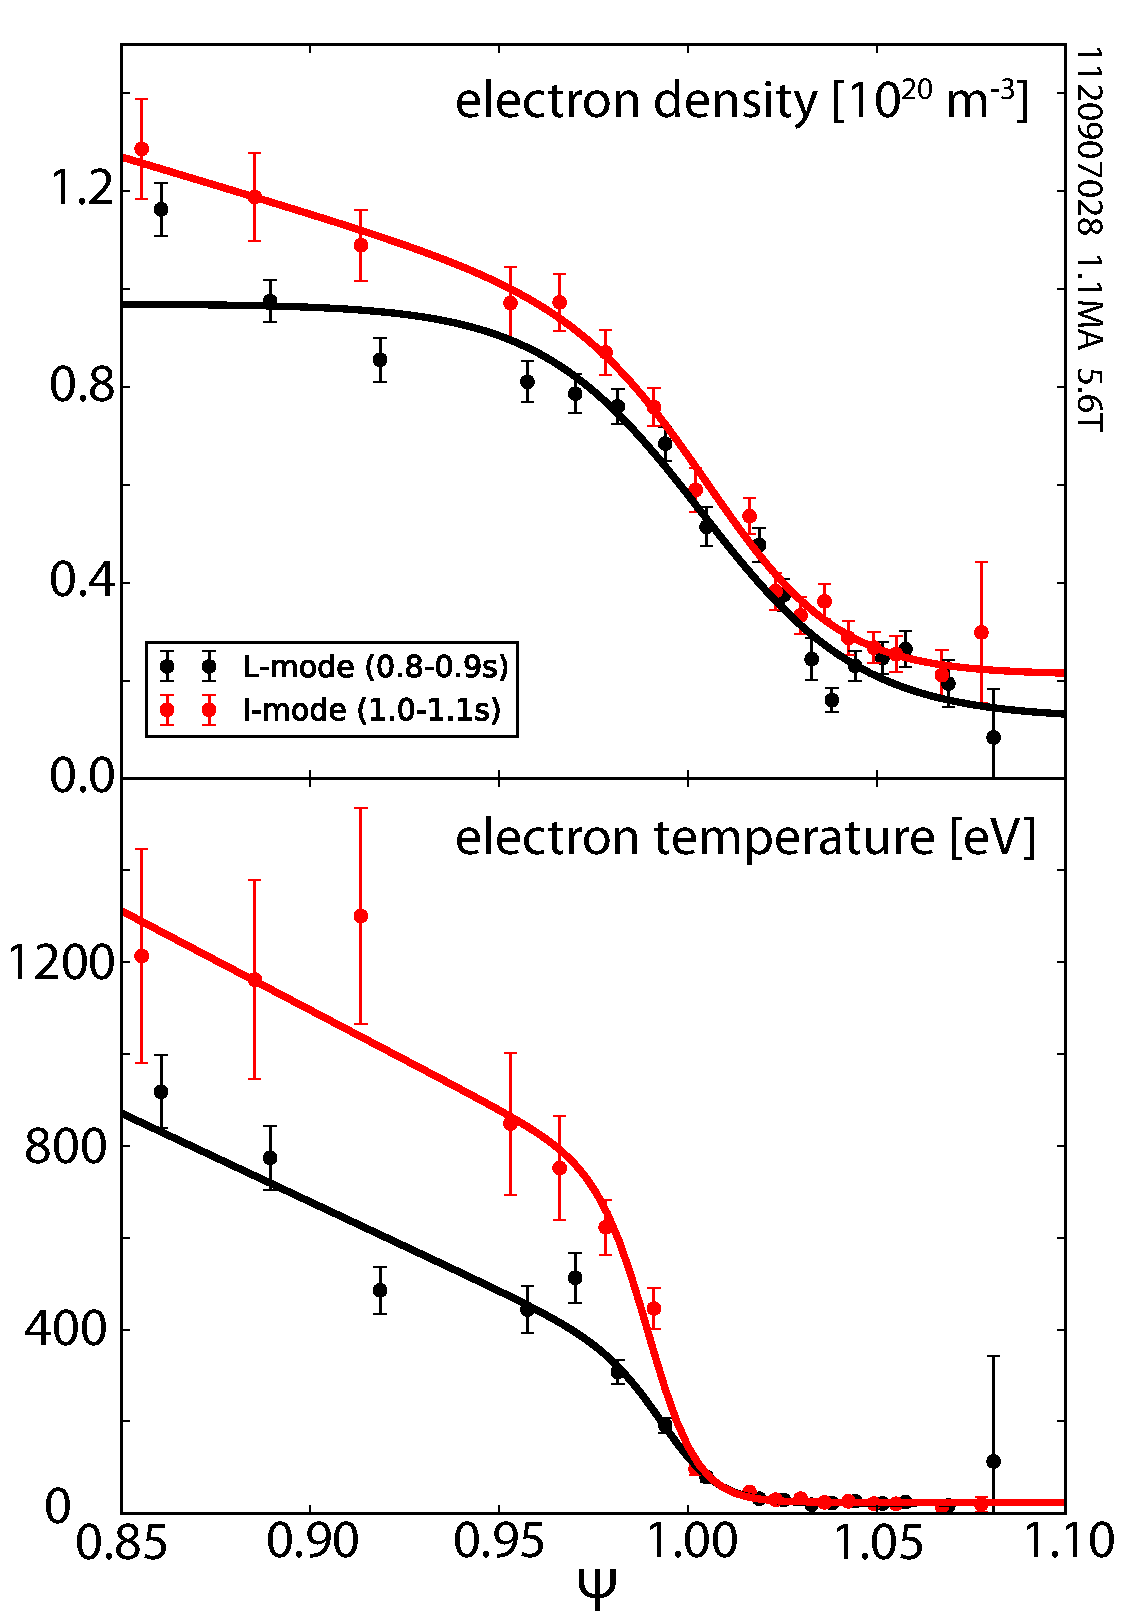
\includegraphics[width=100mm]{graphics/IModePedestal/1120907028_dens_temp.pdf}}
%\end{figure}

\begin{figure}[t]
 \pushtooutside
 \ffigbox[\FBwidth]{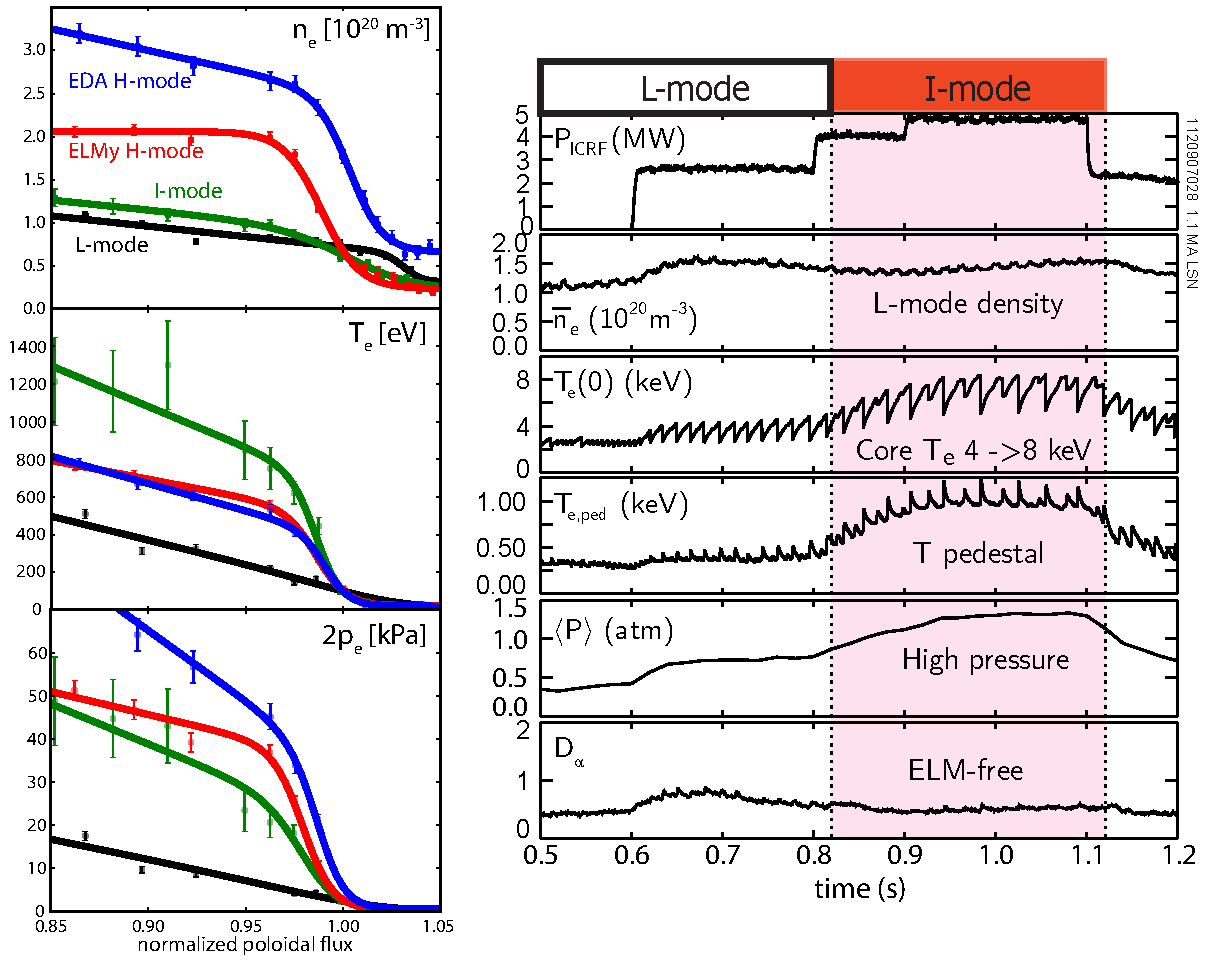
\includegraphics[width=150mm]{graphics/HighPerformanceRegimes/trace_imode.pdf}}{\caption[Characteristic traces for a typical I-mode, and comparisons of I-mode pedestal profiles to L- and H-modes.]{(left) Characteristic traces for a typical I-mode.  At the L-I transition, the core and edge temperature rise over several sawtooth cycles before reaching a steady level; global confinement and pressure rise accordingly.  However, the density remains at L-mode levels, and no ELMs are exhibited.  (right) Edge profiles for density, temperature, and pressure in L-, I-, and H-mode.  The I-mode (green) retains an density profile comparable to the L-mode (black), unlike the ELMy (red) and EDA (blue) H-modes which form a strong density pedestal.  However, the I-mode forms a higher temperature pedestal than either H-mode.  As a result, the I-mode reaches comparable pedestal pressures to the H-modes while retaining L-mode particle transport. (repeated from \cref{fig:hcr_imode_trace})}\label{fig:imode_trace_ped}}
\end{figure}

A firm understanding of the pedestal is essential for the extrapolation of any high-performance regime to ITER- and reactor-scale devices.  The pedestal height sets a strong constraint on core temperature and pressure -- and therefore overall fusion performance -- both by acting as a boundary condition for the plasma profiles, and by supporting steeper core temperature gradients due to profile stiffness \cite{Kinsey2011,Hubbard1998}.  Moreover, the pedestal structure, particularly the steep gradients in density, temperature, and/or pressure, determines stability of the plasma against large, deleterious ELMs (see \cref{sec:mod_pb}).  In this chapter, we present empirical observations of the pedestal in I-mode from a recent series of dedicated experiments \cite{Walk2014}, with a focus on high-resolution pedestal profile measurements across a range of plasma parameters.  Through this, we examine trends in I-mode pedestal behavior, and their impact on global behavior and performance in I-mode, and possible extrapolations to larger devices.\nicesectionending

\section{Access and Experimental Setup}\label{sec:imode_setup}

\begin{figure}[p]
 \pushtooutside
 \fcapside[60mm]{\caption[I-mode edge safety collisionality and safety factor.]{Range in edge collisionality $\nu^*_{95}$ and $q_{95}$ over which I-modes have been accessed.  Notably, I-mode operation is naturally favored near ITER targets for these parameters.  The subset of this data prepared with high-resolution pedestal profiles, herein termed the ``pedestal database'', is also highlighted.}\label{fig:imode_q_nustar}}{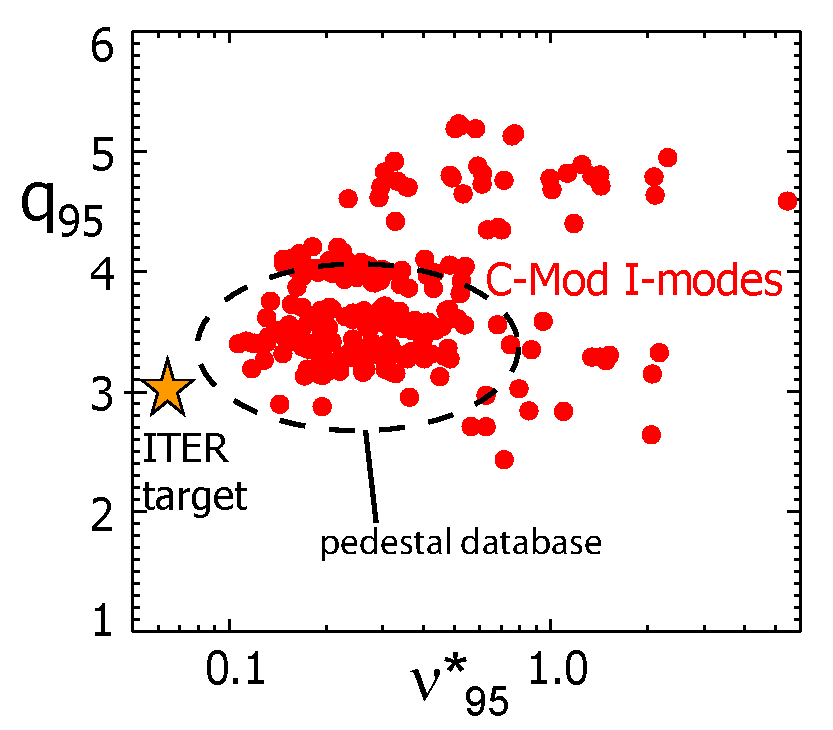
\includegraphics[width=100mm]{graphics/IModePedestal/q95_vs_nustar_2012_Imodeonly.pdf}}
\end{figure}

\begin{figure}[p]
 \pushtooutside
 \fcapside[60mm]{\caption[Density and power range for I-mode access]{Line-averaged density and loss power range for USN and LSN I-modes, illustrating $\sim 2 \times P_{L-I}$ range for $1-\SI{1.2}{\mega\ampere}$, $5-\SI{6}{\tesla}$ I-modes.  USN shapes are forward-field and LSN-shapes are reversed field, such that all I-modes shown are in the unfavorable drift configuration.  \note{swap for plot showing only high-res database, or highlight range?}}\label{fig:imode_p_nebar_access}}{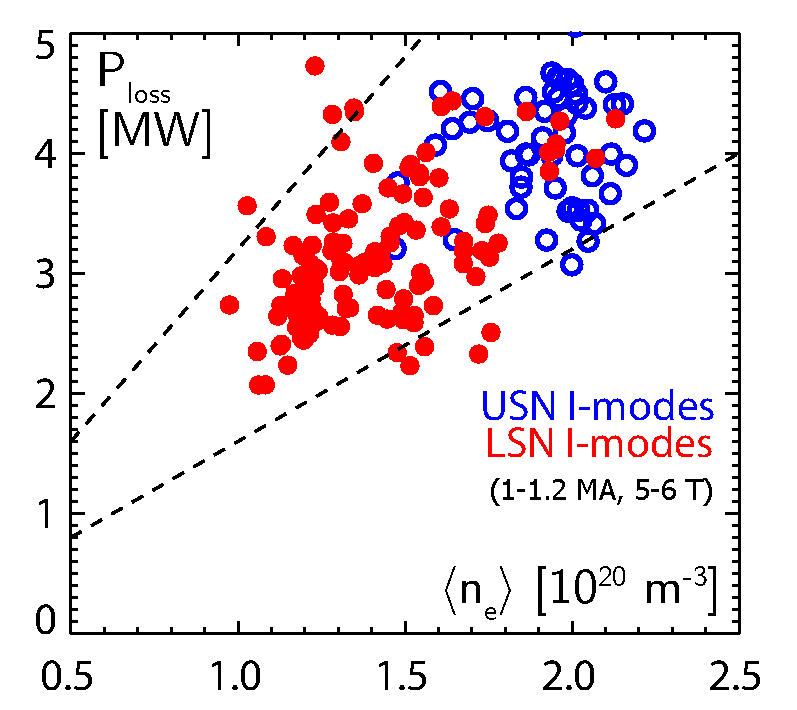
\includegraphics[width=100mm]{graphics/IModePedestal/Ploss_nebar_2013.pdf}}
\end{figure}

%\begin{figure}[p]
% \pushtooutside
% \fcapside[60mm]{\caption[Density and power range for I-mode access]{Line-averaged density and loss power range for I-modes in the pedestal database, illustrating $\sim 2 \times P_{L-I}$ range for $1-\SI{1.2}{\mega\ampere}$, $5-\SI{6}{\tesla}$ I-modes.}\label{fig:imode_p_nebar_access}}{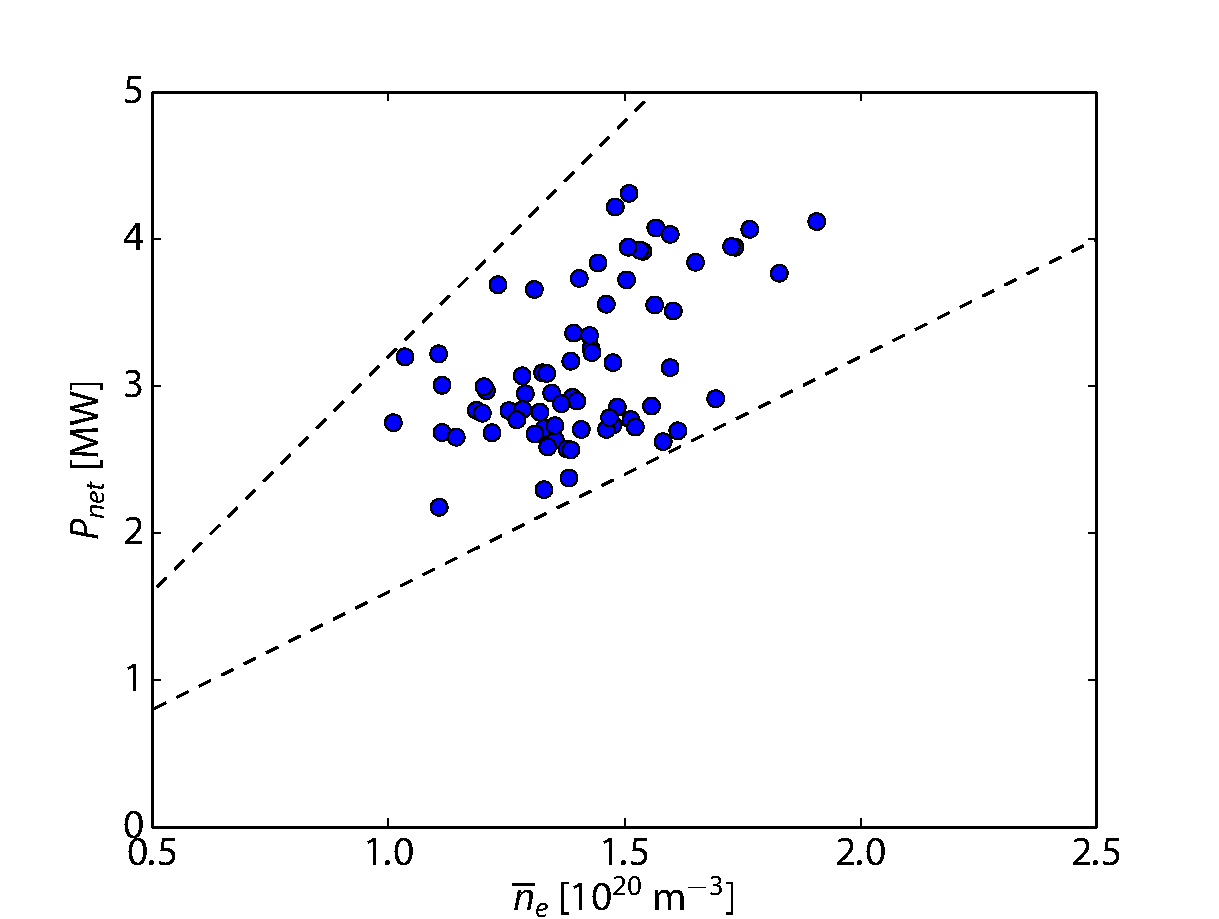
\includegraphics[width=100mm]{graphics/IModePedestal/nebar_Pnet.pdf}}
%\end{figure}

All data presented here was taken on the Alcator C-Mod tokamak, described in \cref{sec:intro_cmod}.  As described in \cref{subsec:hcr_imode_access}, I-mode access hinges primarily on operation with the ion $\nabla B$ drift (\cref{eq:gradbdrift}) directed away from the primary X-point in the plasma (the ``unfavorable $\nabla B$ drift'' configuration).  Within this requirement, though, I-mode access is fairly robust, with steady I-modes sustained in a variety of shapes -- both USN with standard field, and LSN shapes with reversed field to achieve the desired $\nabla B$ drift direction (in the latter case, the plasma current is reversed as well to preserve field helicity) -- and edge-current profiles, and at low-to-moderate collisionality (\cref{eq:nustar}).  The attained range in $q_{95}$ and $\nu^*_{95}$ is shown in \cref{fig:imode_q_nustar}.  I-mode has been sustained with heating power up to $\sim 2 \times$ the L-I transition threshold power, which tends to increase approximately linearly with density (see \cref{fig:imode_p_nebar_access}), above which the plasma typically enters an ELM-free H-mode (recall that operating with unfavorable $\nabla B$ drift elevates the H-mode threshold power by roughly a factor of two \cite{Suttrop2003,Carlstrom1998,Groebner1998}).

I-mode experiments in the 2012 run campaign have focused on reversed-field LSN plasmas, which exhibit the widest access window and avoid difficulties with power handling and edge diagnostics.  A subset of results from these experiments have been prepared with high-resolution pedestal measurements, optimized for analysis of the I-mode pedestal structure both from an empirical standpoint and for a computational approach to the pedestal stability; these data, herein termed the ``pedestal database'' (parameter range highlighted in \cref{fig:imode_q_nustar}) is stored in an SQL database (see \cref{app:sql}) for easy access and analysis, and will be used for the bulk of the I-mode work in this thesis (\cref{ch:ImodePedestal,ch:ImodeModeling}).\nicesectionending

\section{Pedestal Responses}\label{sec:imode_height}

To understand the physics of the I-mode pedestal, it is useful to compare the I-mode to established scalings for baseline H-modes.  For the purposes of this discussion, we distinguish between the \emph{MHD-limited} pedestals found in ELMy H-mode (see \cref{sec:hcr_elmy}) and the \emph{transport-limited} pedestals in EDA H-mode (see \cref{subsec:hcr_eda}).  The pedestal structure in the MHD-limited case is determined by peeling-ballooning stability, described in \cref{sec:mod_pb} -- this manifests predominantly as a limit on the pressure gradient due to the instability drive for the ballooning mode, $\alpha_{MHD}$ (see \cref{eq:alphaMHD,eq:alphaMHD_cyl}).  This scales as $\alpha_{MHD} \sim \nabla p / B_p^2$, consistent with the observed $\nabla p \sim I_p^2$ dependence observed in experiments \cite{Walk2012,Groebner2013} (\cf \cref{ch:Elmy}).  To lowest-order approximation, this sets a limit on the pedestal poloidal beta, such that for a given current, field, and shaping configuration the pedestal pressure $p \sim n_e T_e$ is fixed.  Altering the density via fueling results in heating or cooling the pedestal to maintain this limit, while attempts to modify the pedestal via heating power alters the energy transport (increasing the ELM frequency $f_{ELM} \sim P$ for large type-I ELMs \cite{Urano2003}).  In transport-limited EDA H-mode pedestals, on the other hand, the pedestal is controlled in part by the interplay between the strong particle pinch and the continuous outward particle transport driven by the QCM, such that the density tends to lock to a value set by the plasma current.  Within this limit, the pedestal temperature (and therefore pressure) responds positively to increased heating power \cite{Hubbard2001}.

\subsection{Pedestal Temperature}\label{subsec:imode_temp}

As the I-mode is characterized, in part, by its H-mode-like temperature pedestal and energy confinement, that is a suitable place to begin an examination of the I-mode pedestal.  A scan of plasma current from $\num{0.85}$ to $\SI{1.35}{\mega\ampere}$ reveals a positive trend of the pedestal temperature with plasma current, shown in \cref{fig:imode_Ip_Te95} with ELMy H-modes for comparison.  The I-mode temperature pedestal meets or exceeds the pedestal $T_e$ found in H-modes.  This is highly beneficial for global performance, as the high temperature pedestal coupled with stiff core temperature profiles supports very high (up to $\SI{8}{\kilo\electronvolt}$) core temperatures -- with moderately peaked core density profiles, this supports comparable core pressures and fusion reaction rates to H-mode despite the reduced pedestal pressure (see \cref{subsec:imode_pres}).

\begin{figure}
 \pushtooutside
 \fcapside[60mm]{\caption[Pedestal temperature vs. plasma current for I-mode and ELMy H-mode.]{Pedestal temperature versus plasma current for I-mode and ELMy H-mode.  I-mode temperature pedestals meet or exceed H-mode levels, and trend positively with current.  The spread in $T_{e,95}$ at a given current point is due to varying power per particle (see \cref{fig:imode_Pnebar_Te95}).  The highest-current I-modes exhibit temperatures below the bulk trend due to low values of $P_{net}/\overline{n}_e$, as these I-modes were fueled to relatively high densities.}\label{fig:imode_Ip_Te95}}{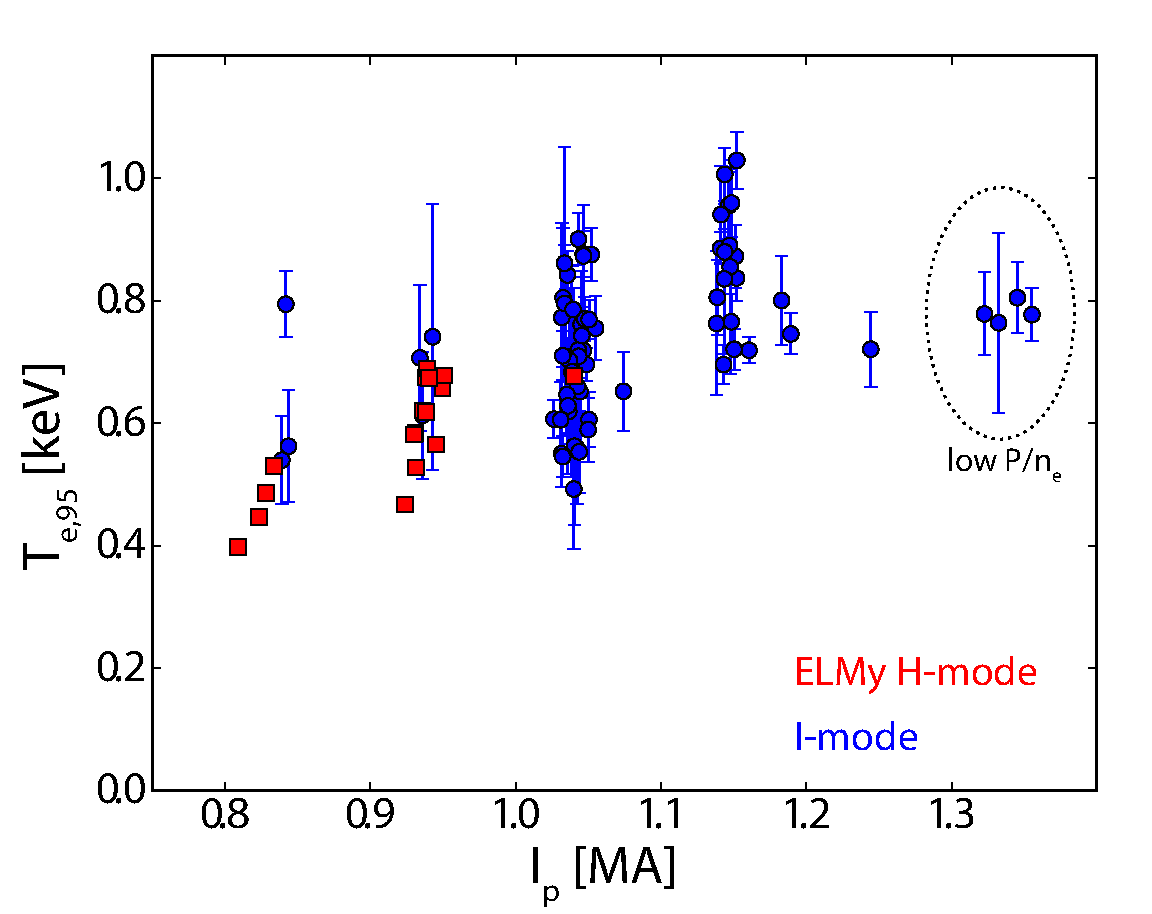
\includegraphics[width=100mm]{graphics/IModePedestal/Ip_Te95.pdf}}
\end{figure}

There is, however, significant scatter at a given point in the $I_p$ scan, due to variation in the input heating power.  Examining a single current slice at $\SI{1.15}{\mega\ampere}$, shown in \cref{fig:imode_Pnebar_Te95}, we see a strong dependence of the temperature pedestal height on the net heating power (\cref{eq:pnet}), normalized to (line-averaged) density -- effectively, the input power per particle.  This same pattern is observed at other current points.  The comparatively suppressed temperatures at the highest-current I-modes is a result of the higher fueling at these points, resulting in lower values of $P_{net}/\overline{n}_e$.  I-modes in these experiments were typically fueled to densities corresponding to Greenwald fractions  (\cref{eq:GDL}) $0.15 \le f_{Gr} \le 0.26$, with the highest-current points at $f_{Gr} \sim 0.2$, or $\SI{1.8e20}{\per\meter\cubed}$.

\begin{figure}
 \pushtooutside
 \fcapside[60mm]{\caption[Pedestal temperature vs. heating power per particle for an example current slice.]{Pedestal temperature $T_{e,95}$ vs. heating power per particle ($P_{net}/\overline{n}_e$) for the $\SI{1.15}{\mega\ampere}$ current slice, illustrating the approximately-linear trend in temperature at fixed current.  This behavior is highly beneficial as an external control for the pedestal temperature.}\label{fig:imode_Pnebar_Te95}}{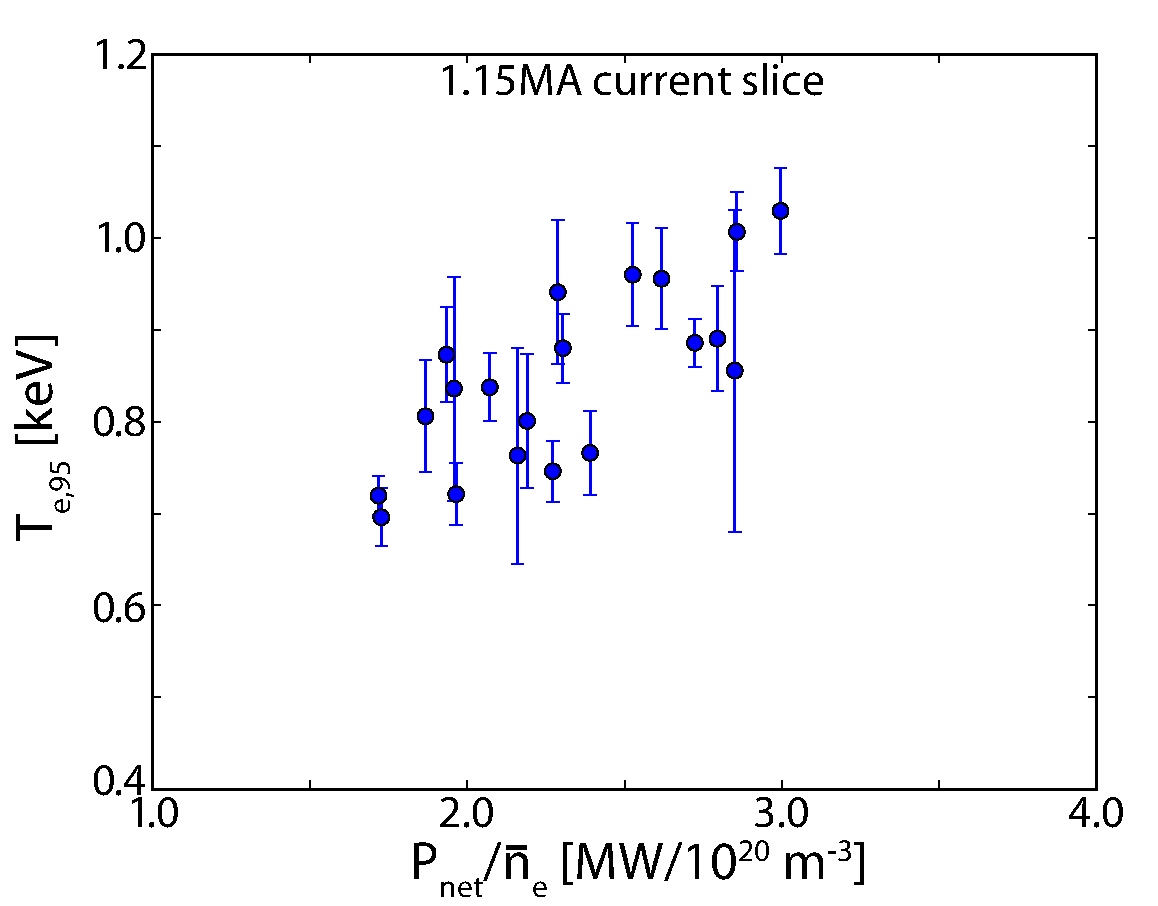
\includegraphics[width=100mm]{graphics/IModePedestal/Pnebar_Te95_115MA.pdf}}
\end{figure}

The temperature pedestal response in I-mode to plasma current is comparable to that seen in the density, temperature, and pressure pedestals in ELMy H-mode (\cf \cref{fig:elmy_ipscan}), although the sensitivity of the temperature pedestal in ELMy H-mode is somewhat weaker than in I-mode.  The response of the temperature pedestal to heating power is notable: the temperature in ELMy H-mode pedestals is only weakly dependent on power -- rather, increased heating power increases the ELM frequency and energy transport to maintain the approximately $\beta_p$-limited pedestal (\cf \cref{fig:hcr_elmybetas,fig:elmy_neBp_TeBp}).  Transport-limited EDA H-mode pedestals exhibit a similar trend, given as $T_{e,ped} \sim \left(P_{net}/\overline{n}_e\right)^{0.5 \pm 0.1}$ in \cite{Hubbard2001} and $T_{e,ped} \sim \left(P_{net}/n_{e,L}\right)^{0.7 \pm 0.1}$ in \cite{Hughes2002}, with the I-mode pedestal responding at least as strongly -- this suggests that I-mode pedestals are not stability-limited. 

\subsection{Pedestal Response to Fueling}\label{subsec:imode_fueling}

In contrast to the temperature pedestal (\cref{subsec:imode_temp}), the edge density in I-mode exhibits markedly different behavior compared to conventional H-modes.  Edge density is set primarily through operator fueling control via gas puffing, maintaining an L-mode-like density profile without the density pedestal found in H-mode.  The pedestal response to fueling is shown at right in \cref{fig:imode_density}.  Compared to transport-limited EDA pedestals, the plasma current is insufficient as a predictor of I-mode pedestal density, with the positive trend (shown at left in \cref{fig:imode_density}) due to the strong co-variance between $I_p$ and $\overline{n}_e$.

\begin{figure}[ht]
 \pushtooutside
 \ffigbox[\FBwidth]{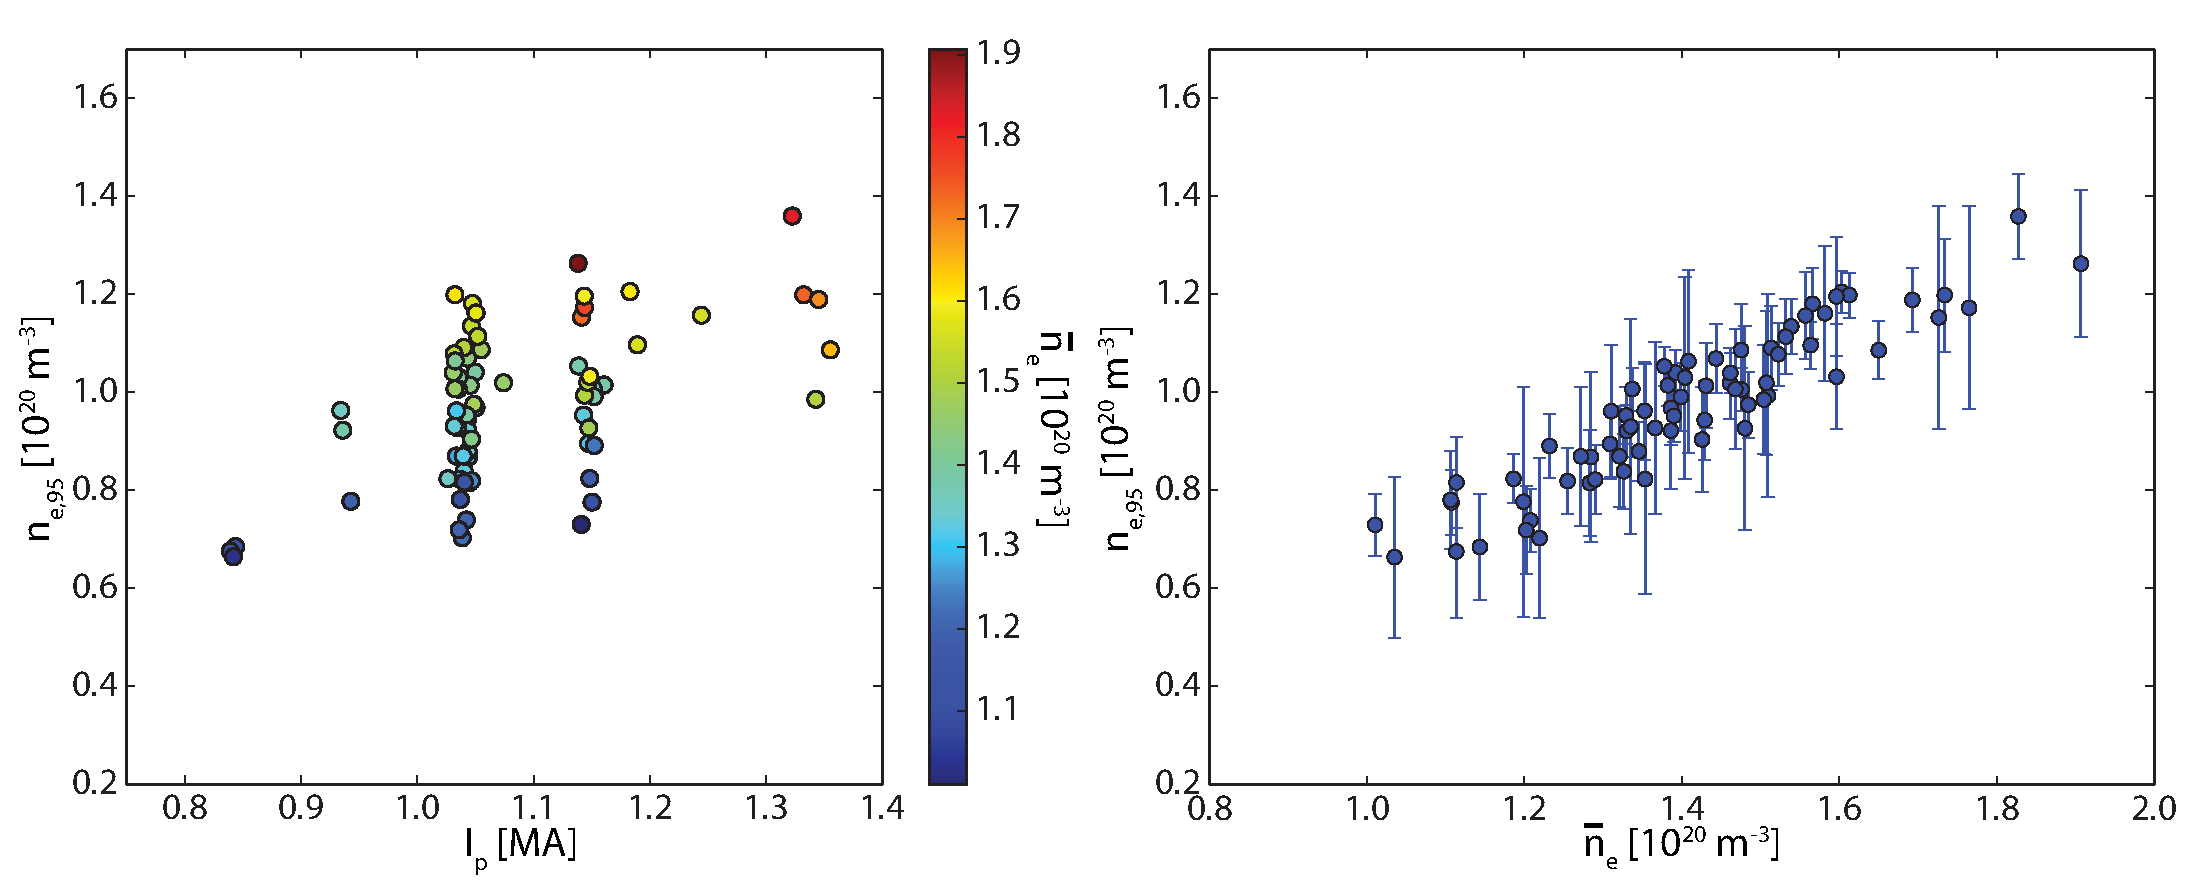
\includegraphics[width=150mm]{graphics/IModePedestal/imode_density.pdf}}{\caption[Pedestal density response to current and fueling.]{Pedestal density as a function of current (left, colored by $\overline{n}_e$) and line-averaged density (right).  The pedestal density is set solely by operator fueling; in contrast the transport-limited pedestals in EDA H-mode, plasma current is a poor predictor of the pedestal density, with the trend due only to the co-variance between $I_p$ and $\overline{n}_e$.}\label{fig:imode_density}}
\end{figure}

\begin{figure}[ht]
 \pushtooutside
 \fcapside[60mm]{\caption[Density and temperature pedestals at matched current and field with varying fueling and heating power -- matched $P_{net}/\overline{n}_e$ maintains the $T_e$ pedestal.]{Density and temperature pedestals at matched current, field, and shaping, with varying fueling and heating power levels.  The three discharges are fueled to $\overline{n}_e$ of $\num{1.0}$ (black), $\num{1.3}$ (blue), and $\SI{1.7e20}{\per\meter\cubed}$ (red) respectively, with heating powers of $\num{2.75}$, $\num{3.65}$, and $\SI{4.10}{\mega\watt}$ to maintain matched $P_{net}/\overline{n}_e \sim 2.4-2.7$.  The constant power-per-particle maintains matched temperature pedestals across the fueling range, indicative of the independent control of pedestal $n_e$ and $T_e$ available in I-mode.}\label{fig:imode_fuelingprofiles}}{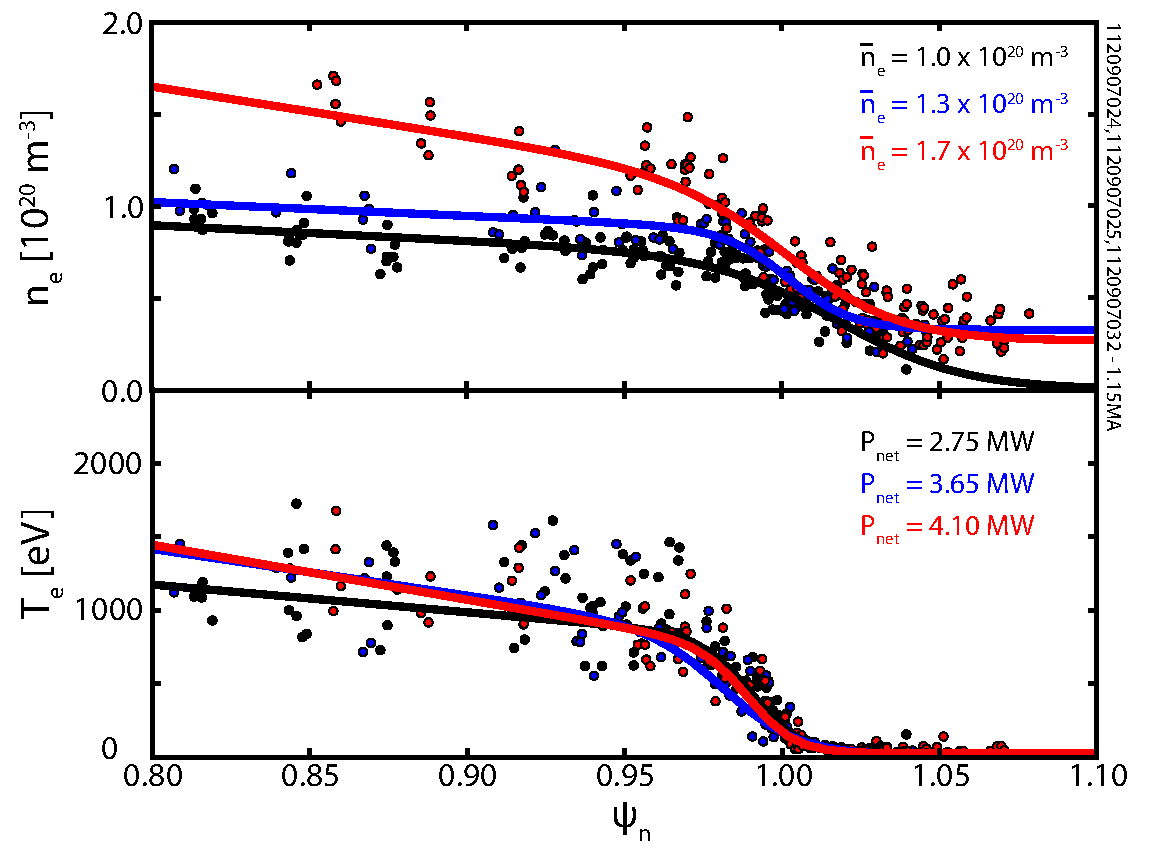
\includegraphics[width=100mm]{graphics/IModePedestal/fuelingprofiles.pdf}}
\end{figure}

Given sufficient heating power, temperature pedestals can be maintained with increased density due to the strong response of $T_{e,95}$ to power-per-particle.  Example discharges matched in current, field, and shaping are shown in \cref{fig:imode_fuelingprofiles}, spanning a range in fueling and heating power, $\overline{n}_e = 1.0 - \SI{1.7e20}{\per\meter\cubed}$, $P_{net} = 2.75 - \SI{4.10}{\mega\watt}$.  Temperature pedestals are matched across all three discharges, using consistent power-per-particle $P_{net}/\overline{n}_e = 2.4 - \SI{2.7}{\mega\watt}/10^{20}\;\si{\per\meter\cubed}$.

This behavior is distinct from that found in H-modes on C-Mod.  ELMy H-modes at fixed current and shaping exhibit an inverse relationship between pedestal $n_e$ and $T_e$ due to limited pedestal $\beta_p$, such that increased fueling tends to cool the pedestal (although the modification of pedestal collisionality also modifies the ELM character).  EDA H-modes lack the fueling control found in I-mode, instead railing the pedestal density to a value set by the plasma current, such that the outward transport and strong inward particle pinch are balanced.  The largely-decoupled behavior of the density and temperature profiles in the edge in I-mode are highly desirable from an operational standpoint -- fueling (done entirely via edge gas puffing on C-Mod) and heating power are separated as ``knobs'' for plasma and pedestal control, granting significant operational freedom compared to the relatively-constrained H-mode pedestal behavior.

The phenomenon demonstrated in \cref{fig:imode_fuelingprofiles} is indicative of a path to strongly improved performance in I-mode, increasing pedestal $\beta_p$ and global confinement via matched increases in fueling and heating power, maintaining the target temperature pedestal with appropriate levels of $P_{net}/\overline{n}_e$.  Recent experiments on C-Mod \cite{Hubbard2012} have successfully applied this approach, reaching elevated density by fueling into an established I-mode in combination with increased heating power levels, reaching heating power levels that would trigger a transition to H-mode in a comparable-density L-mode.\gnote{L-mode-like fueling with turbulent pinch, get Kesler paper?}

\begin{figure}[h]
 \pushtooutside
 \fcapside[60mm]{\caption[Pedestal pressure versus plasma current in I-mode and ELMy H-mode.]{Pedestal thermal pressure ($2 \times p_{e,95}$) versus plasma current, colored by fueling level indicated by line-averaged density $\overline{n}_e$.  The shaded region indicates the typical range of pedestal pressures in C-Mod ELMy H-modes.  A strong, roughly $p_{95} \sim I_p$ trend in pedestal pressure is observed.  At a given current, a strong increase in pedestal pressure with fueling is also observed (note: heating power also varied in these discharges).}\label{fig:imode_Ip_p95}}{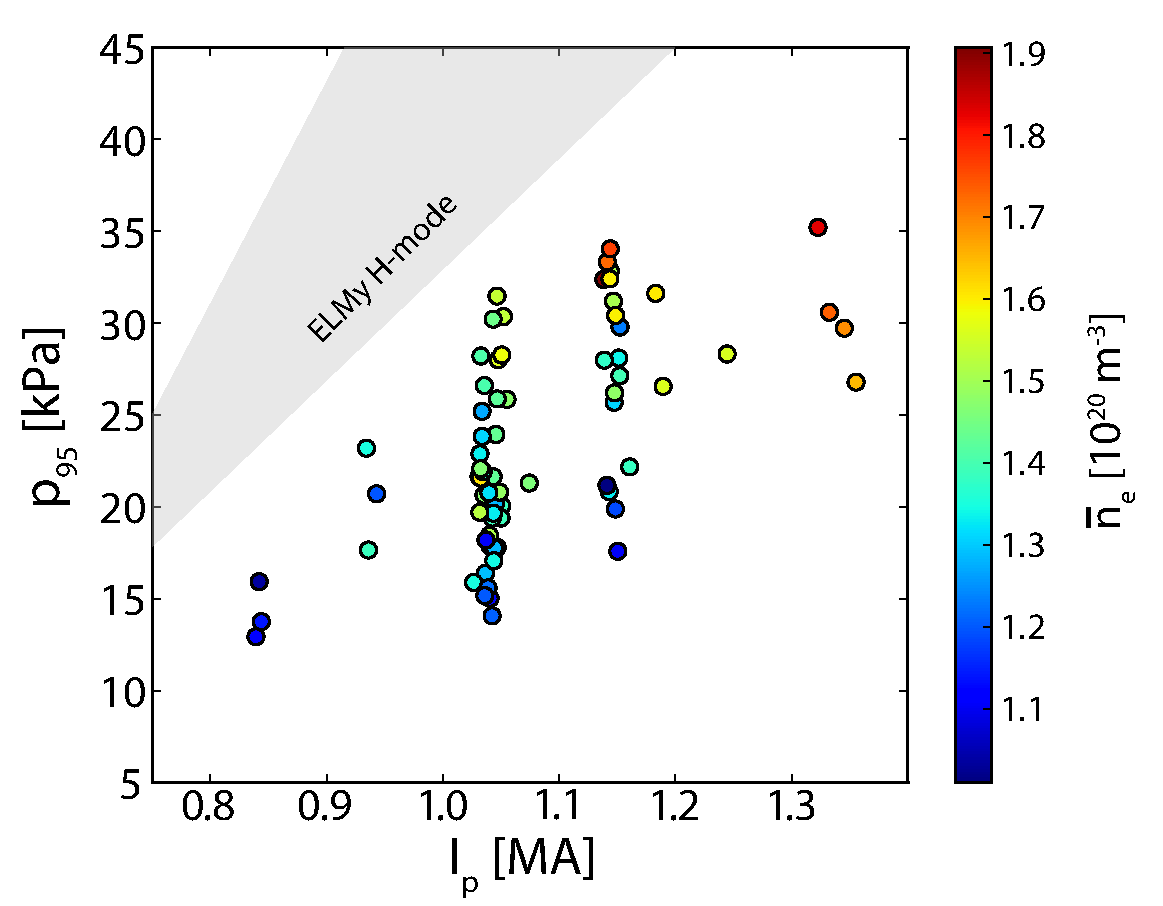
\includegraphics[width=100mm]{graphics/IModePedestal/Ip_p95_nebar.pdf}}
\end{figure}

\subsection{Pressure Pedestal Scalings and Performance}\label{subsec:imode_pres}

Despite lacking a density pedestal, I-mode is capable of reaching pedestal thermal pressures comparable to H-mode, while maintaining favorable behavior  in its particle (particularly impurities -- see \cref{fig:hcr_imode_taui}) transport and temperature pedestal.  I-mode pedestal pressure (we use twice the electron pressure from Thomson Scattering here, consistent with $T_i \approx T_e$ measurements in well-equilibrated pedestals on C-Mod \cite{Hubbard2011} and with the relatively low impurity contribution to the pressure, $Z_{eff} \sim 2$) versus plasma current is shown in \cref{fig:imode_Ip_p95}, with additional differentiation by fueling level indicated by color.  An increase in pedestal pressure by at least $p_{95} \sim I_p$ is observed, consistent with the scaling of the temperature pedestal $T_e \sim I_p$.  The pedestal pressure at a given current is seen to increase strongly with increased fueling, consistent with the maintenance of the temperature pedestal with increased heating power and matched fueling, thus constant levels of $P_{net}/\overline{n}_e$.  I-mode pedestal pressure is reduced from that typically found in H-mode (the typical range in ELMy H-mode is indicated by the shaded region in \cref{fig:imode_Ip_p95}).  This is due to the reduced pedestal density in I-mode compared to H-mode, as the temperature pedestals found in I-mode typically meet or exceed H-mode levels.  The pressure pedestal is expected to be ultimately limited by the ELM trigger -- however, the indepedent density and temperature pedestal control should allow I-mode to approach, but not exceed, the ELMing limit.

The effect of heating power on the pressure pedestal is visible in \cref{fig:imode_Pnet_p95}, showing the $\SI{1.15}{\mega\ampere}$ current slice (see \cref{fig:imode_Pnebar_Te95} for the same).  At fixed current, the pressure pedestal scales as $p_{95} \sim P_{net}$, consistent with the previously observed $T_{e,95} \sim P_{net}/\overline{n}_e$ trend in the temperature pedestal as $p_{95} \sim n_{e,95} T_{e,95}$.  This corresponds the favorable scaling of energy confinement in I-mode with heating power -- plasma stored energy is set by heating power and the energy confinement time, $W \sim P \tau_E$, and is strongly influenced by the pedestal pressure (see \cref{fig:imode_p95_W}).  Thus, the trend $p_{95} \sim P_{net}$ is consistent with little or no degradation of $\tau_E$ with heating power, which has been observed in global measurements of I-mode \cite{Dominguez2012,Whyte2010}, and is distinct from the trend $\tau_E \sim P^{-0.7}$ found for ELMy H-modes \cite{ITER1999}.  This behavior is quite favorable when scaled to large, high-power machines, particularly in scenarios with a significant degree of fusion self-heating, where the plasma pressure directly determines heating power via the fusion reaction rate ($\sim p^2$).

\begin{figure}[t]
 \pushtooutside
 \fcapside[60mm]{\caption[Pedestal pressure vs. heating power for an example current slice.]{Pedestal pressure ($2\times p_{e,95}$) versus net heating power for the $\SI{1.15}{\mega\ampere}$ current slice, illustrating the trend $p_{95} \sim P_{net}$ at fixed current.  This is consistent with the power trend in the I-mode temperature pedestal, $T_{e,95} \sim P_{net}/\overline{n}_e$.}\label{fig:imode_Pnet_p95}}{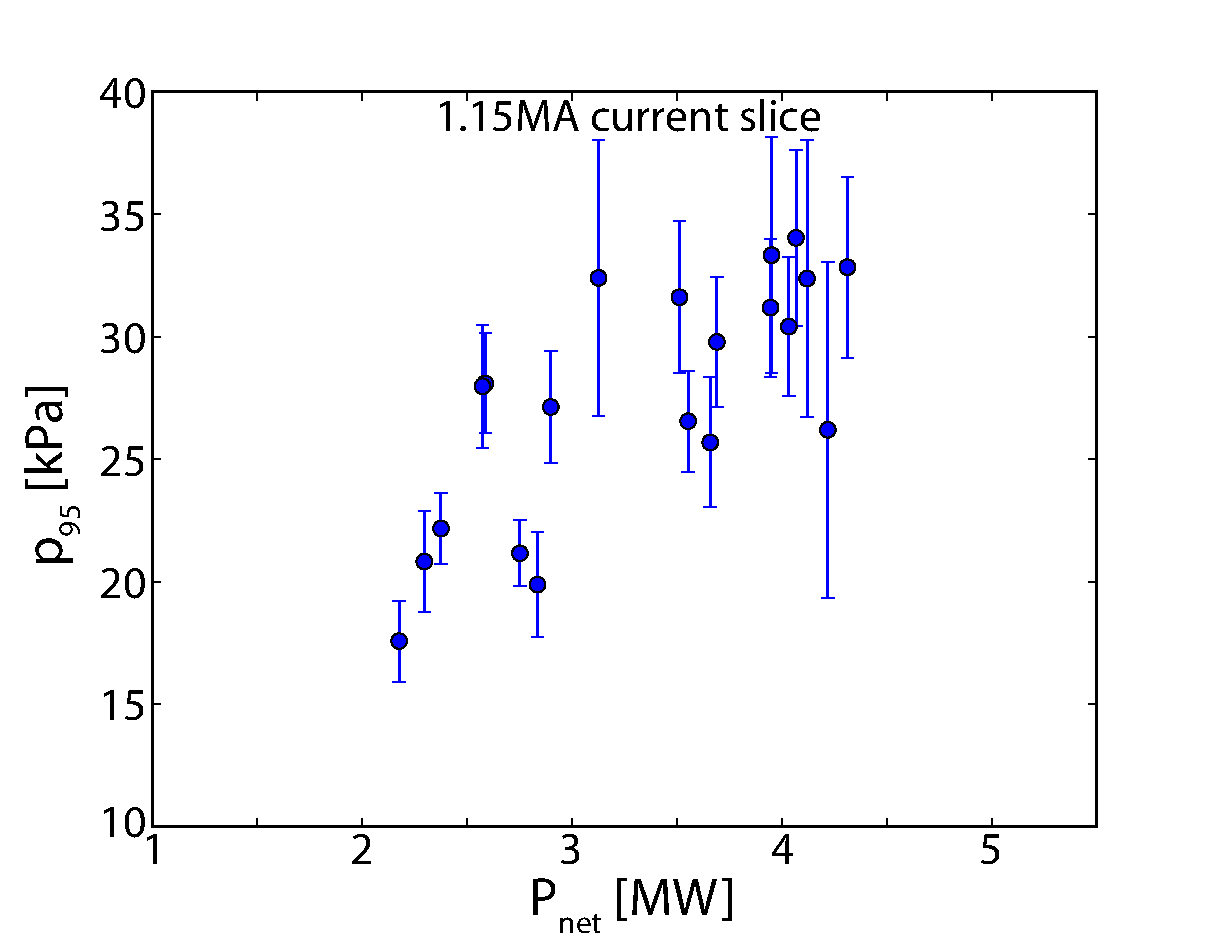
\includegraphics[width=100mm]{graphics/IModePedestal/Pnet_p95_115MA.pdf}}
\end{figure}

\begin{figure}[t]
 \pushtooutside
 \fcapside[60mm]{\caption[Stored energy versus pedestal pressure.]{I-mode stored energy versus pedestal pressure, confirming the strong dependence of global performance on the pedestal height.  \note{N.B. -- may remake figure with ELMy H-modes as well, generally they exhibit lower stored energy at the same pedestal pressure}}\label{fig:imode_p95_W}}{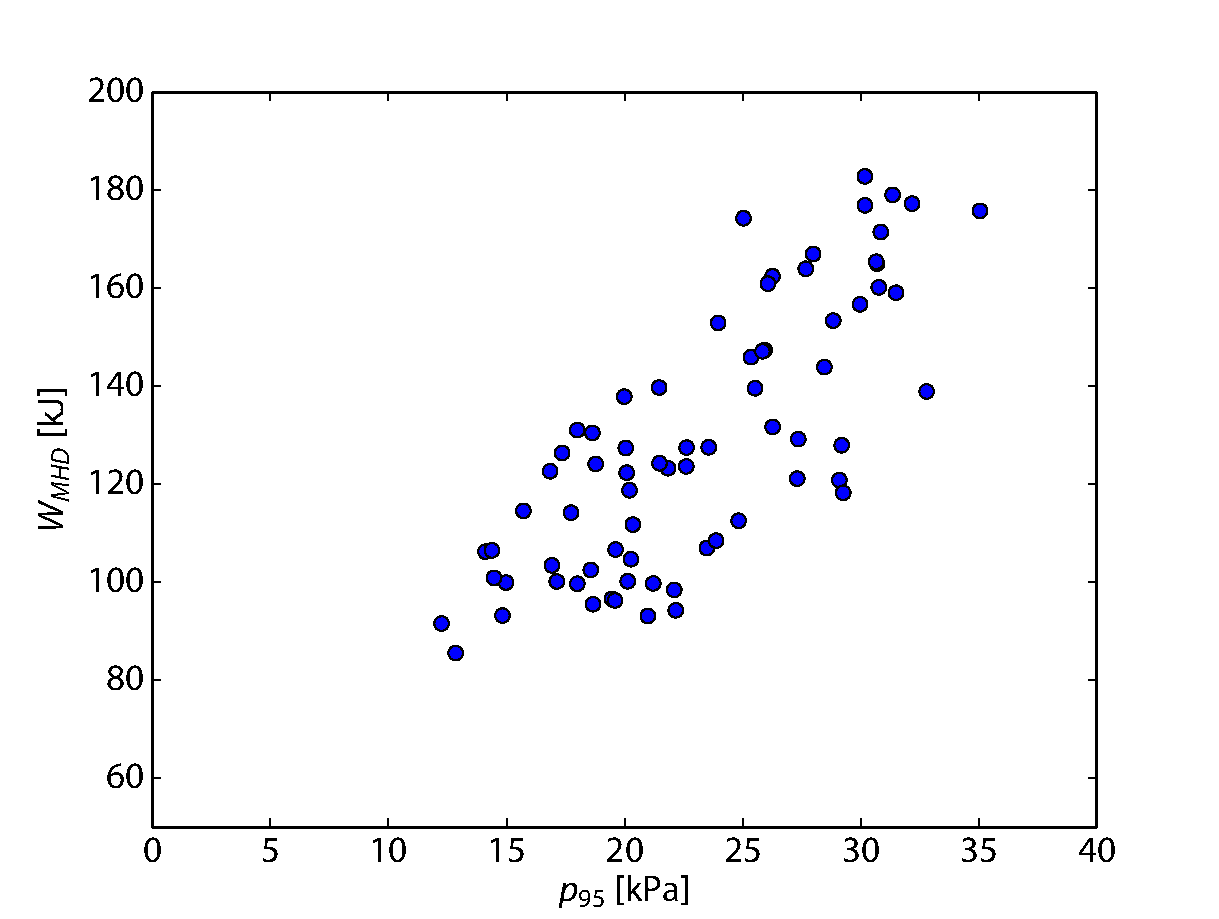
\includegraphics[width=100mm]{graphics/IModePedestal/p95_W.pdf}}
\end{figure}

Trends in the pressure pedestal in I-mode are also informative to its MHD stability.  As shown in \cref{fig:imode_ip_gradp}, the peak pressure gradient (identified as the driver for ballooning MHD instabilities, described in \cref{subsec:mod_balloon}, and the trigger for large ELMs) in I-mode is consistently shallower at a given $I_p$ than comparable ELMy H-modes on C-Mod, due to the flat edge density profile.  Moreover, the pedestal pressure gradient scales more weakly than the expected $\nabla p \sim I_p^2$ expected from the ballooning stability boundary \cite{Connor1978}.  The intuitive conclusion from this is that I-mode is generally stable to the MHD instabilities identified with the ELM trigger -- the MHD stability and ELM behavior of I-mode is explored in detail in \cref{ch:ImodeModeling}.\nicesectionending

\begin{figure}[t]
 \pushtooutside
 \fcapside[60mm]{\caption[Pressure gradient vs. plasma current for I-mode and ELMy H-mode.]{Peak pressure gradient (measured at the pedestal midpoint) versus plasma current for I-mode and ELMy H-mode.  I-mode consistently exhibits a weaker pressure gradient at a given current, as well as scaling more weakly than the $\nabla p \sim I_p^2$ expected from the ballooning MHD stability limits associated with ELMy H-mode.}\label{fig:imode_ip_gradp}}{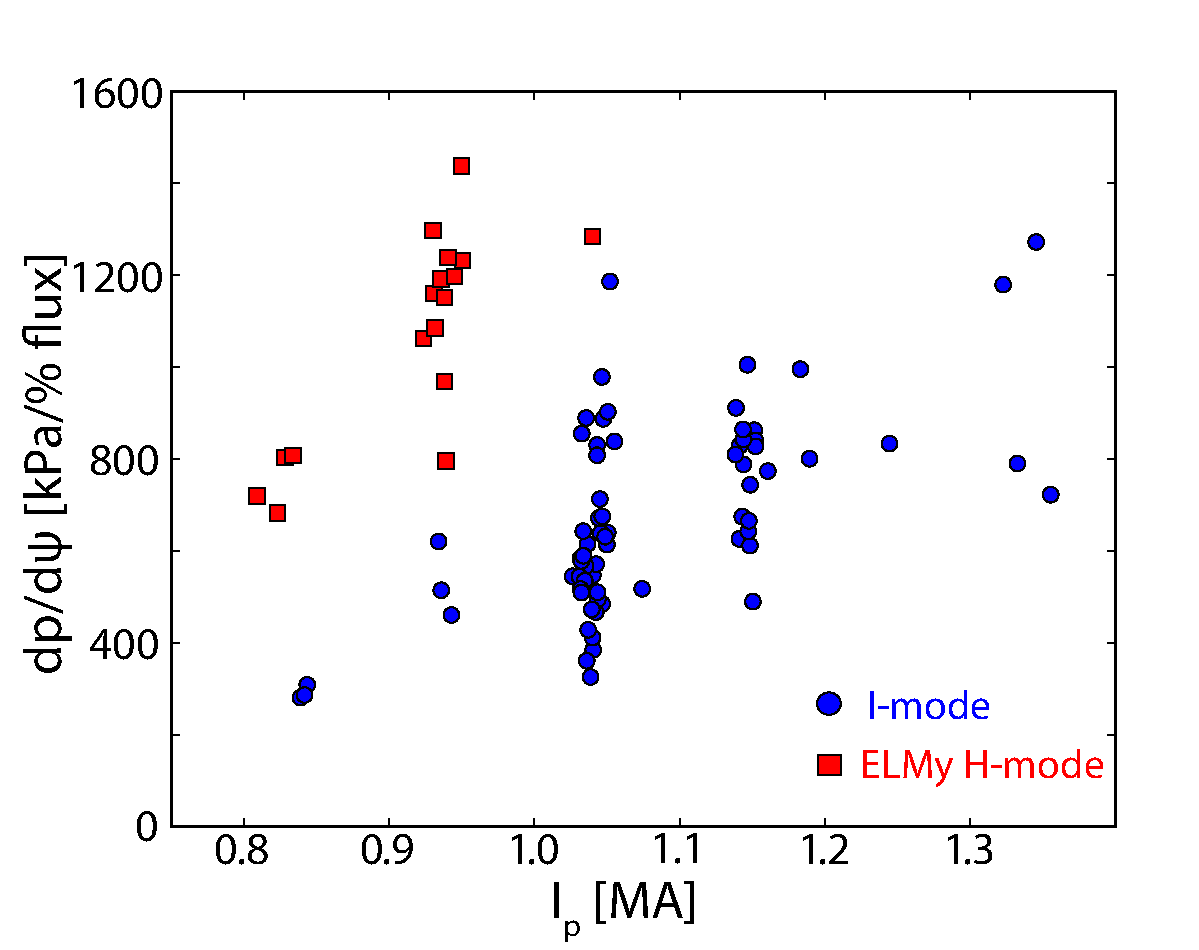
\includegraphics[width=100mm]{graphics/IModePedestal/Ip_gradp.pdf}}
\end{figure}

\section{Pedestal Widths}\label{sec:imode_width}

Conventionally, H-mode pedestals are found to be constrained by critical-gradient-driven instabilities, such that the peak $\nabla p$ is limited -- therefore, the width of the transport barrier sets a constraint on the attainable pedestal height (and thus global performance).  Due to the small spatial scales inherent in the pedestal, accurate measurement of the pedestal width has historically been quite difficult, although a number of theoretical models have been proposed and tested against experimental observations, \eg \cite{Maggi2010,Beurskens2011,Onjun2002}.  This section explores a range of potential explanations for the observed pedestal widths in I-mode.

\subsection{Kinetic-Ballooning Limited Pedestals}\label{subsec:imode_kbm}

%The edge turbulence in I-mode is characterized by a strong reduction in mid-frequency turbulence and the appearance of a higher-frequency ($\sim 200 - \SI{400}{\kilo\hertz}$) fluctuation, dubbed the \emph{Weakly-Coherent Mode} or WCM \cite{Whyte2010,Hubbard2011,Dominguez2012,Cziegler2011,Cziegler2013,White2011}.\gnote{not sure I like this intro}  The WCM appears to be connected to the density pumpout and pedestal regulation in I-mode, with the WCM amplitude shown to be correlated to the particle flux through the LCFS \cite{Dominguez2012}.  An understanding of the turbulent behavior in the I-mode pedestal, then, is essential to the extrapolation of I-mode operation to larger devices.  Kinetic-ballooning mode (KBM) turbulence, described in \cref{sec:mod_turbulence}, is thought to constrain the pedestal in ELMy H-mode, and is therefore an important starting point for investigating the WCM.

\begin{figure}[t]
 \pushtooutside
 \fcapside[60mm]{\caption[Pedestal width vs. poloidal beta in I-mode and ELMy H-mode.]{Pedestal width versus poloidal beta in I-mode and ELMy H-mode.  ELMy H-modes lie on the $\Delta_\psi \sim \beta_{p,ped}^{1/2}$ line predicted for KBM-limited pedestals (see \cref{subsec:elmy_eped_width}).  I-mode shows no scaling of the pedestal width with $\beta_p$, and exhibits pedestals consistently wider than predicted for comparable ELM-limited pedestals.}\label{fig:imode_wid_betapol}}{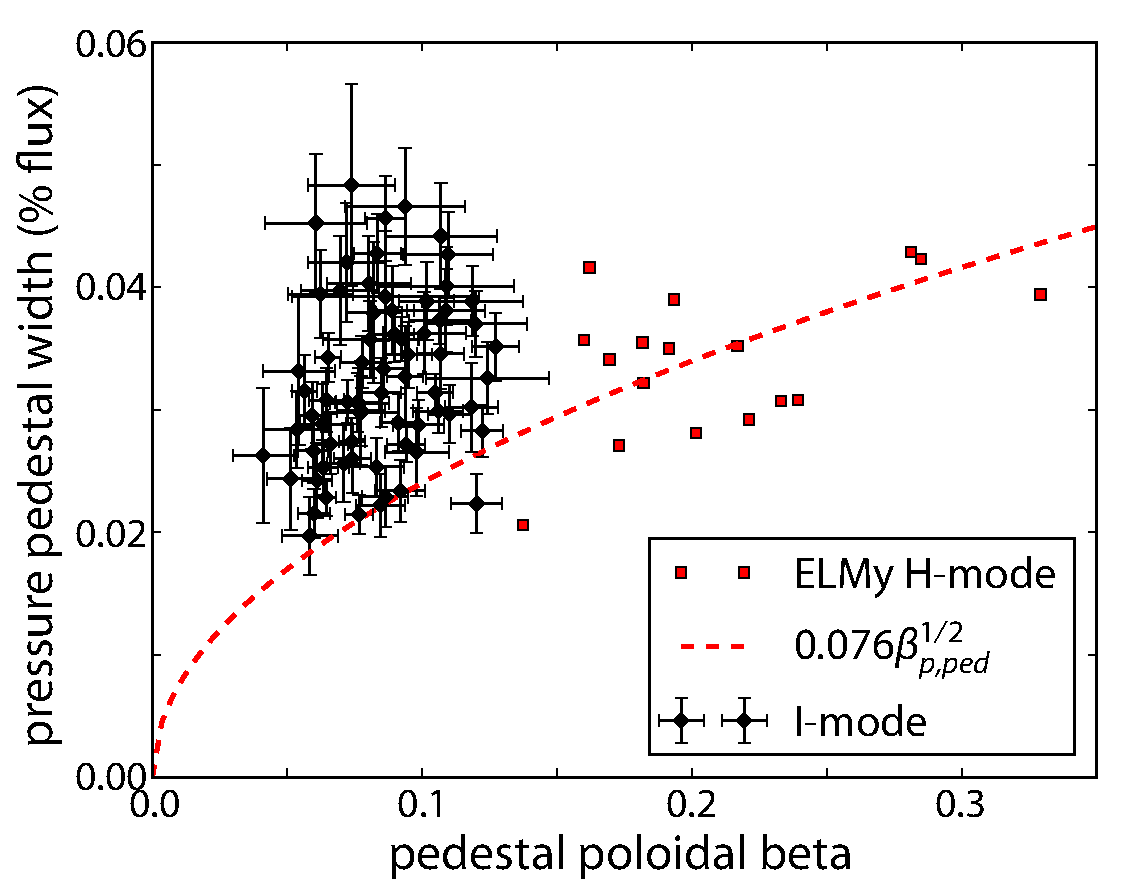
\includegraphics[width=100mm]{graphics/IModePedestal/wid_betapol.pdf}}
\end{figure}

The kinetic-ballooning mode (KBM), described in \cref{sec:mod_turbulence}, applies a constraint to the pedestal width of the form $\Delta \sim \beta_{p,ped}^{1/2}$, where $\Delta$ is the pedestal width in normalized poloidal flux.  This trend has been observed on several machines \cite{Groebner2013,Beurskens2011,Osborne1998}, including on C-Mod (see \cref{ch:Elmy}).  This constraint is used in the EPED model series, described in \cref{sec:mod_eped}.  The simplest implementation of the constraint, used in EPED1 (\cref{subsec:mod_eped1}) uses a fitted coefficient, $\Delta = 0.076 \beta_{p,ped}^{1/2}$ \cite{Snyder2009}.  A comparison of I-mode pedestals against this predictive line, as well as example ELMy H-modes, is shown in \cref{fig:imode_wid_betapol}.  I-mode pedestals are wider on average than predicted by the KBM-limited ($\sim \beta_{p,ped}^{1/2}$) line, and show no trend of pedestal width with poloidal beta.  This suggests that the I-mode pedestal is not constrained by KBM turbulence, consistent with the relaxed pressure gradient found in I-mode -- stability against the KBM is examined in more detail in \cref{sec:imode_baloo}.

\subsection{Local Physics Parameters}\label{subsec:imode_exp_widths}

\begin{figure}[p]
 \pushtooutside
 \ffigbox[\FBwidth]{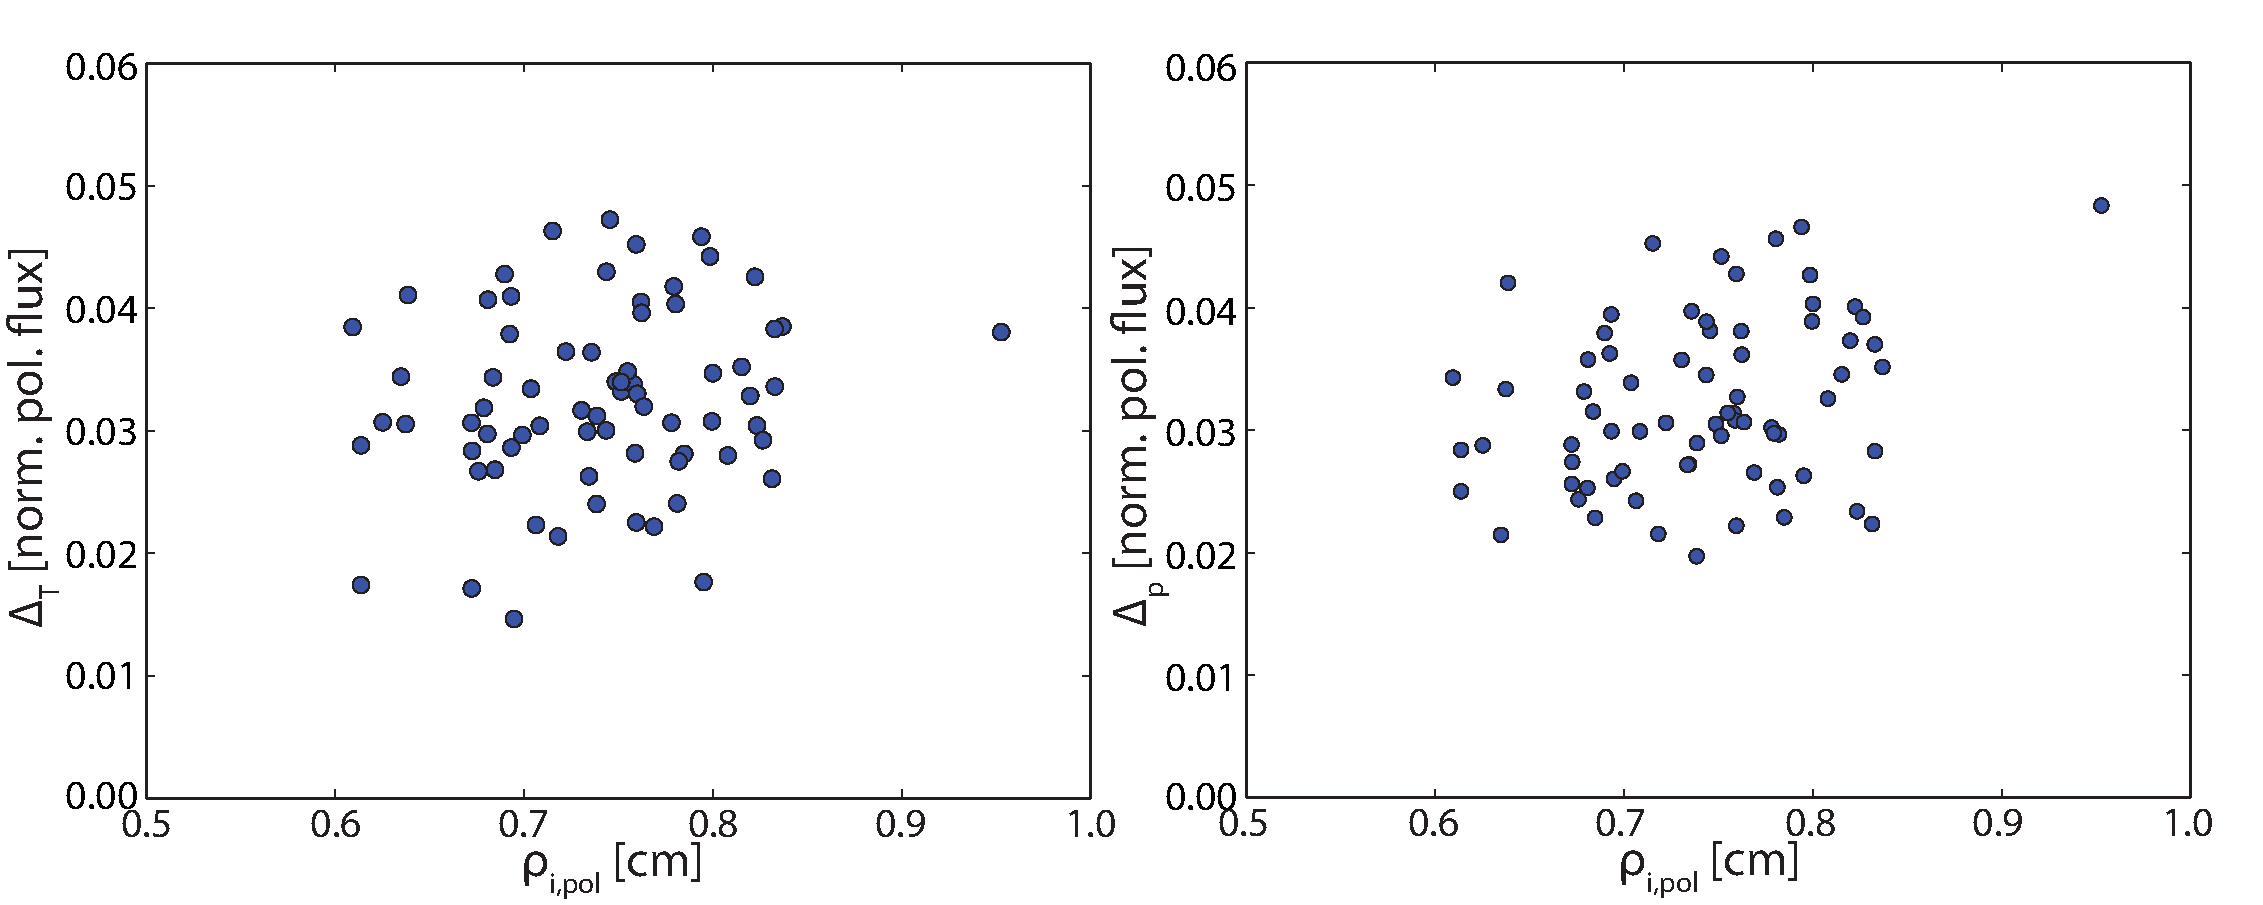
\includegraphics[width=150mm]{graphics/IModePedestal/rhoipol_widths.pdf}}{\caption[Temperature and pressure pedestal width vs. poloidal gyroradius.]{Temperature (left) and pressure (right) pedestal widths versus poloidal gyroradius $\rho_{i,pol}$.  No correlation in the pedestal width is seen, contrary to models suggesting a scaling of the sheared-flow layer and pedestal with the gyroradius.}\label{fig:imode_rhoipol_wid}}
\end{figure}

\begin{figure}[p]
 \pushtooutside
 \ffigbox[\FBwidth]{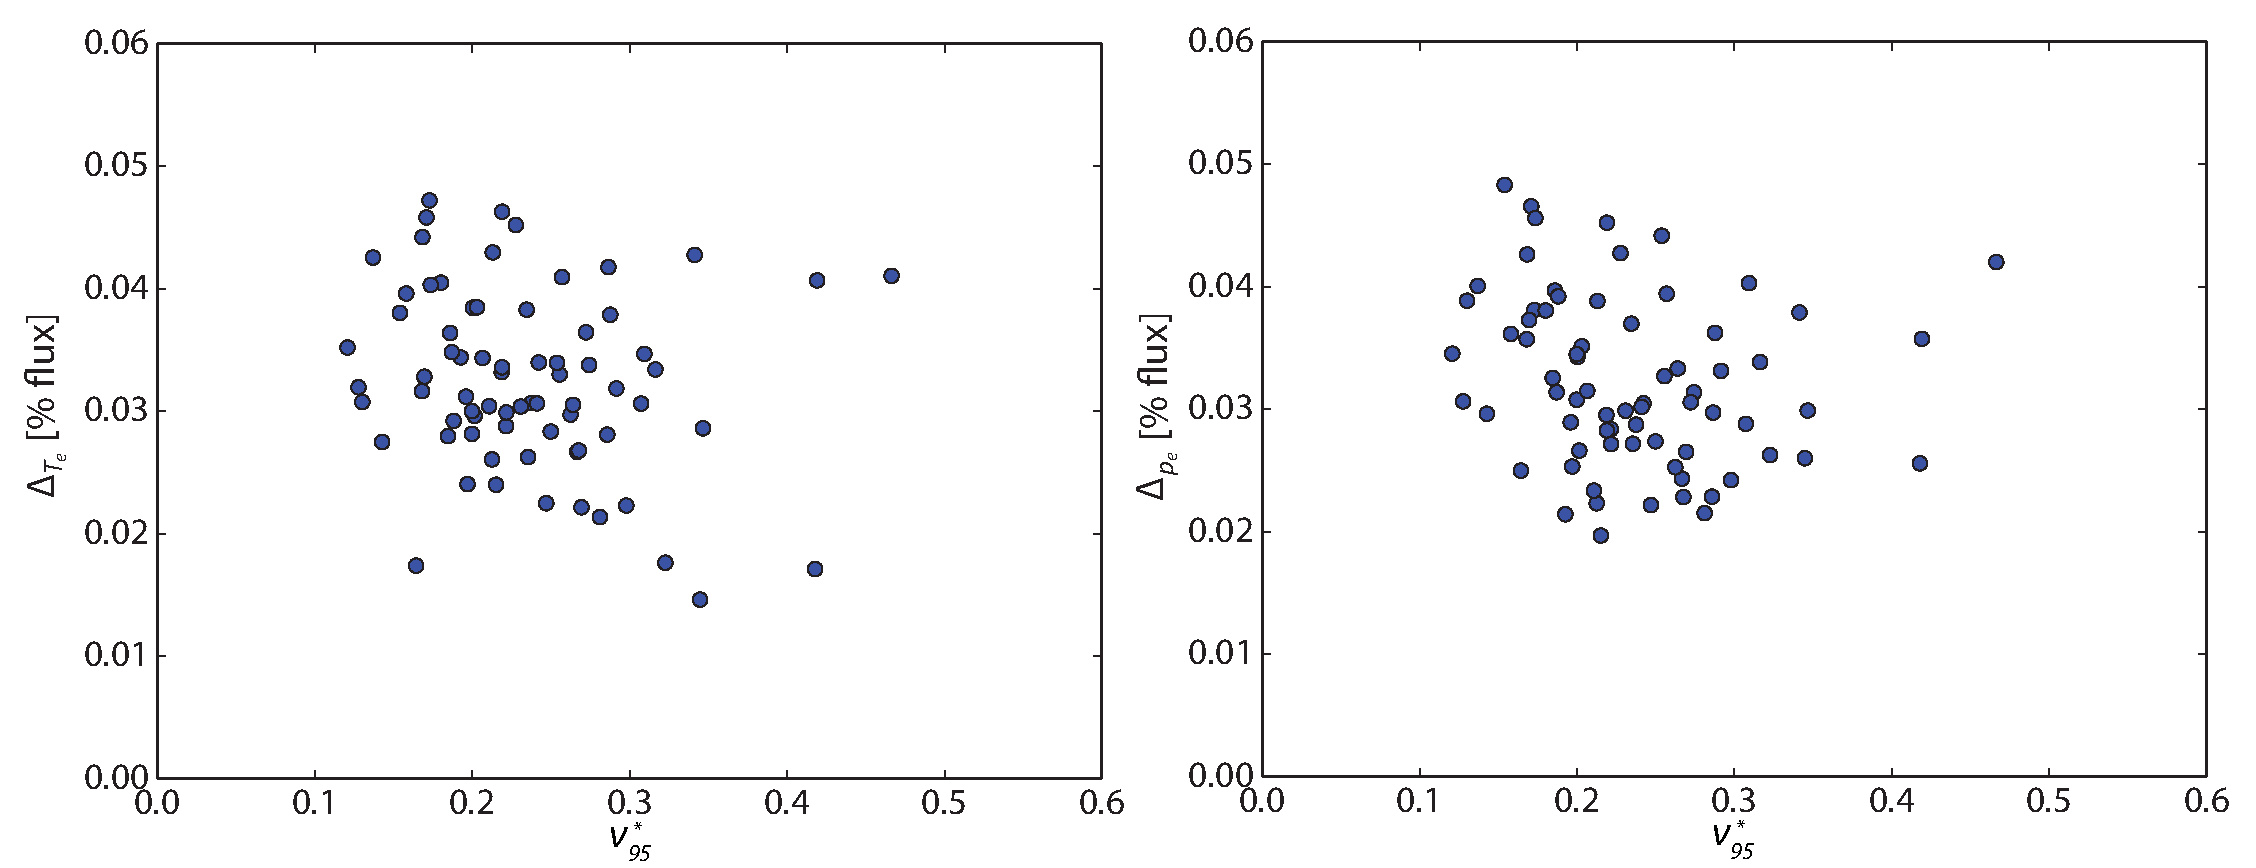
\includegraphics[width=150mm]{graphics/IModePedestal/nustar_widths.pdf}}{\caption[Temperature and pressure pedestal widths vs. pedestal collisionality.]{Temperature (left) and pressure (right) pedestal widths versus pedestal collisionality $\nu^*_{95}$.  No correlation is seen.}\label{fig:imode_nustar_wid}}
\end{figure}

\begin{figure}[p]
 \pushtooutside
 \ffigbox[\FBwidth]{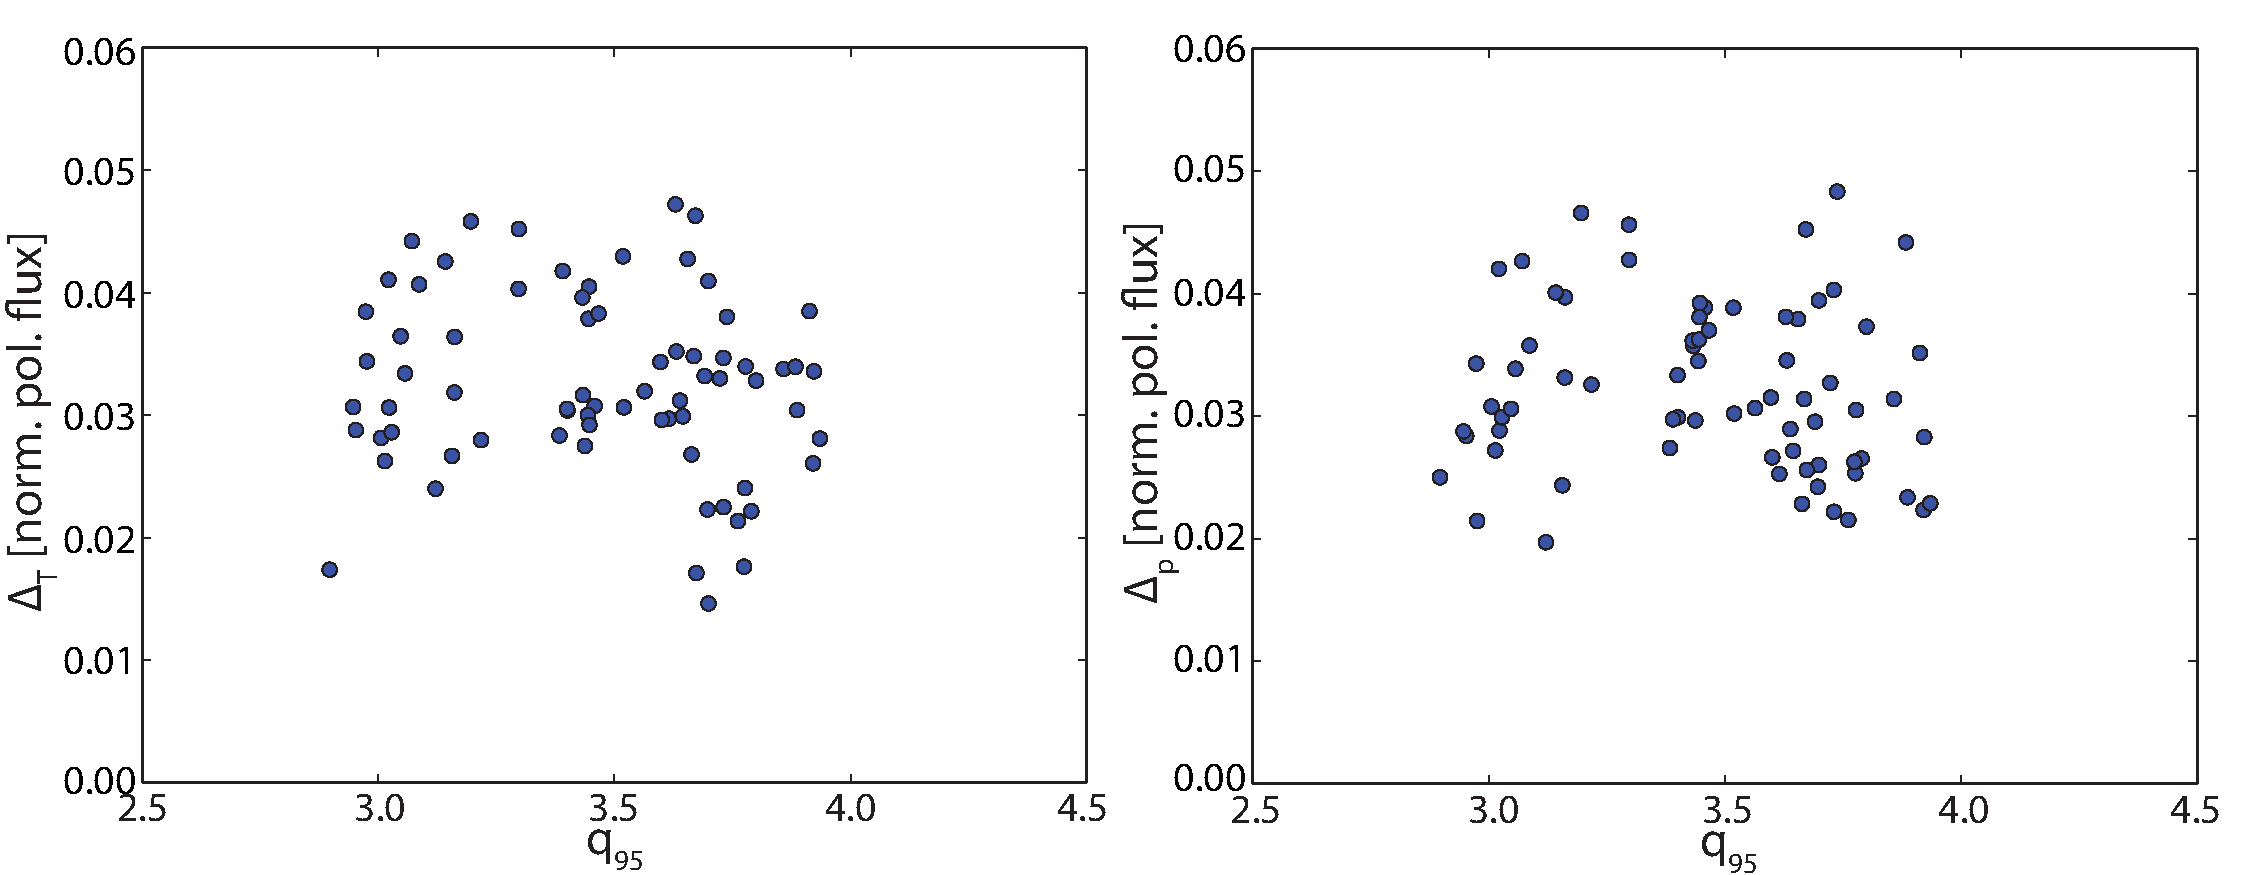
\includegraphics[width=150mm]{graphics/IModePedestal/q95_widths.pdf}}{\caption[Temperature and pressure pedestal widths vs. edge safety factor.]{Temperature (left) and pressure (right) pedestal widths versus edge safety factor $q_{95}$.  No correlation is seen.}\label{fig:imode_q95_wid}}
\end{figure}

While the constraint on the pressure pedestal from kinetic-ballooning turbulence has been the most successful in capturing the limiting physics in ELMy H-modes, a number of other theories (see \cref{sec:mod_early}) based on localized physics in the edge have been proposed, with testable trends in the pedestal width.  Of particular note are models based on a trend in poloidal gyroradius, described in \cref{subsec:mod_ionorbitloss}, operating on the assumption that ion orbit loss in the plasma edge drives the radial electric field responsible for the pedestal formation -- thus the size scale of the ion orbit sets the pedestal width.  Some experimental observations correlate well to these predictions, although these may be largely incidental due to the strong covariance between $\rho_{i,pol}$ and $\beta_{p,ped}$, and have been discounted by dedicated experiments distinguishing the two.  However, as the KBM does not appear to limit the I-mode pedestal (see \cref{subsec:imode_kbm}) gyroradius scalings remain an open avenue.  Electron temperature and pressure pedestal widths are shown against $\rho_{i,pol}$ in \cref{fig:imode_rhoipol_wid}.  Both pedestal widths appear quite insensitive to the gyroradius, although due to the correlation between $T_e$ and $I_p$ the range in $\rho_{i,pol}$ is rather limited.

Similarly, the temperature and pressure pedestal widths are shown against pedestal collisionality $\nu^*_{95}$ and edge safety factor $q_{95}$ in \cref{fig:imode_nustar_wid} and \cref{fig:imode_q95_wid}, respectively.  The collisionality may be expected to influence the pedestal width both by controlling neutral ionization rates (thus the influence of neutral penetration on the pressure width) and through the bootstrap current in the edge, which enters into the peeling-ballooning MHD stability boundary (see \cref{sec:mod_pb}).  The safety factor is directly tied to the magnetic shear, which is locally stabilizing to MHD modes in the edge.  However, as the I-mode pedestal appears to be strongly MHD-stable, as is shown in \cref{ch:ImodeModeling}, these should have a minimal effect.  In \cref{fig:imode_nustar_wid,fig:imode_q95_wid}, no correlation between the pedestal width and either parameter is evident.

In \cref{subsec:imode_temp}, it is shown that the temperature pedestal height is strongly dependent on $P_{net}/\overline{n}_e$, effectively heating power per particle (equivalently, the heat flux through the pedestal).  Temperature and pressure pedestal widths are shown against power-per-particle in \cref{fig:imode_Pnebar_wid}.  As with the other parameters, the pedestal width is uncorrelated with the heat flux through the pedestal.

\begin{figure}[t]
 \pushtooutside
 \ffigbox[\FBwidth]{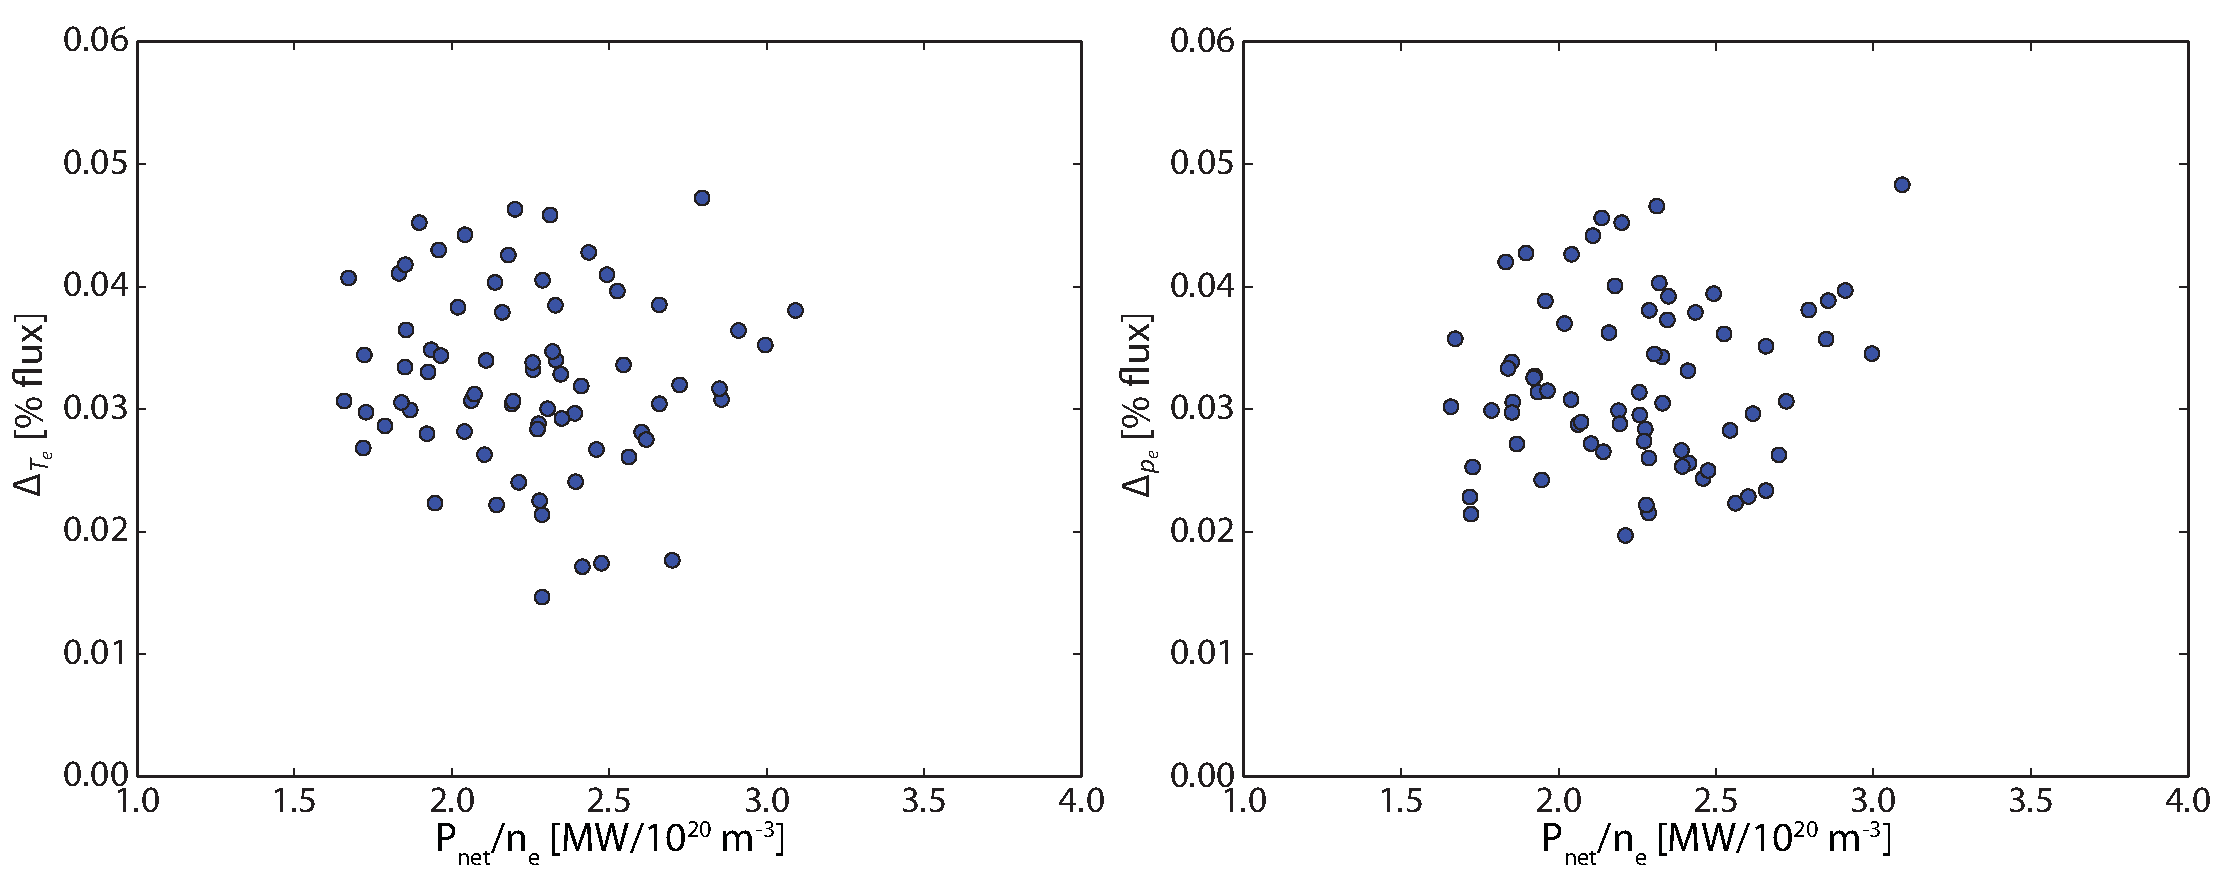
\includegraphics[width=150mm]{graphics/IModePedestal/Pnebar_widths.pdf}}{\caption[Temperature and pressure pedestal width vs. power-per-particle through the pedestal.]{Temperature (left) and pressure (right) pedestal widths versus power-per-particle, $P_{net}/\overline{n}_e$, \ie the heat flux through the pedestal.  No correlation is seen.}\label{fig:imode_Pnebar_wid}}
\end{figure}

\subsection{Stiff Gradient Limits}\label{subsec:imode_wid_stiff}

\begin{figure}[t]
 \pushtooutside
 \fcapside[60mm]{\caption[I-mode pedestal temperature gradient versus pedestal temperature.]{Peak $\nabla T_e$ in the I-mode pedestal versus $T_{e,95}$.  Hotter pedestals support a steeper gradient in temperature (albeit with significant scatter), consistent with a robust temperature pedestal width.}\label{fig:imode_Te_gradT}}{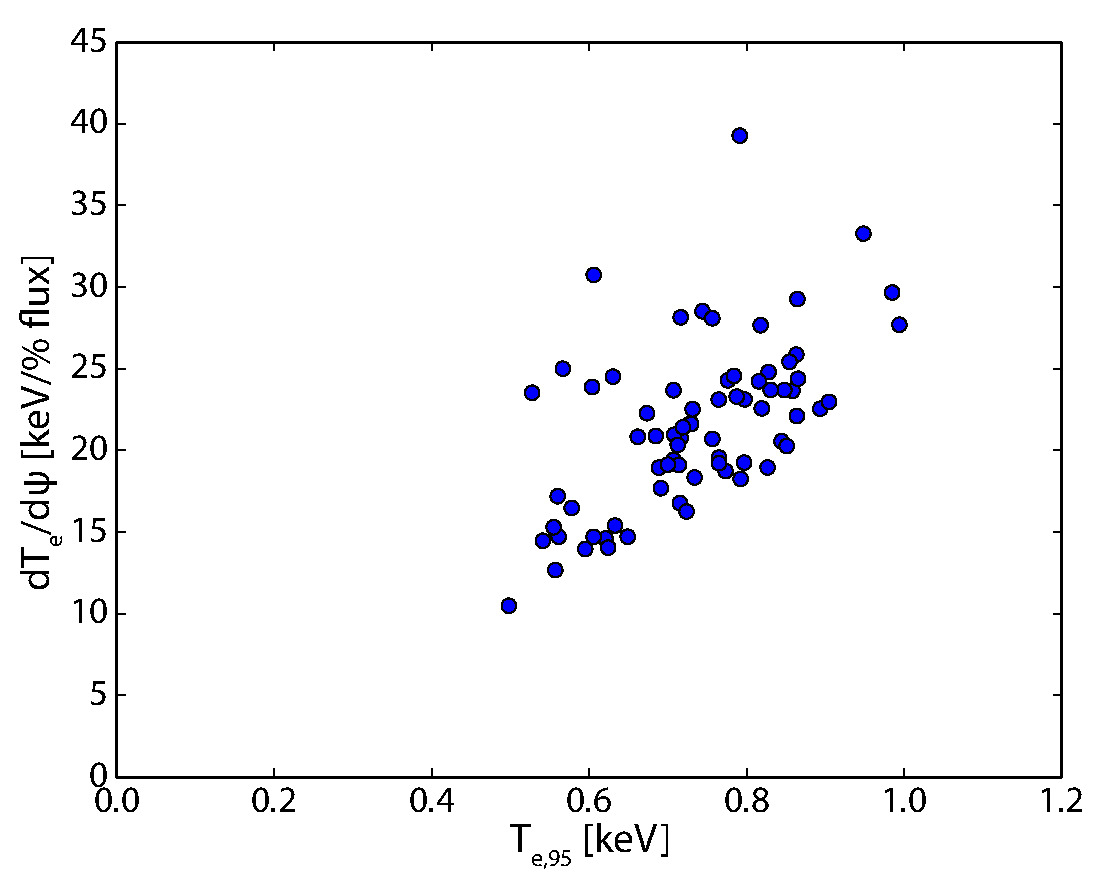
\includegraphics[width=100mm]{graphics/IModePedestal/Te95_gradT.pdf}}
\end{figure}

\begin{figure}
 \pushtooutside
 \fcapside[60mm]{\caption[I-mode pedestal pressure gradient versus pedestal pressure.]{Peak $\nabla p$ in the I-mode pedestal versus $p_{95}$.  There is a robust linear dependence between the pedestal gradient and height, consistent with a robust pedestal width.}\label{fig:imode_p_gradp}}{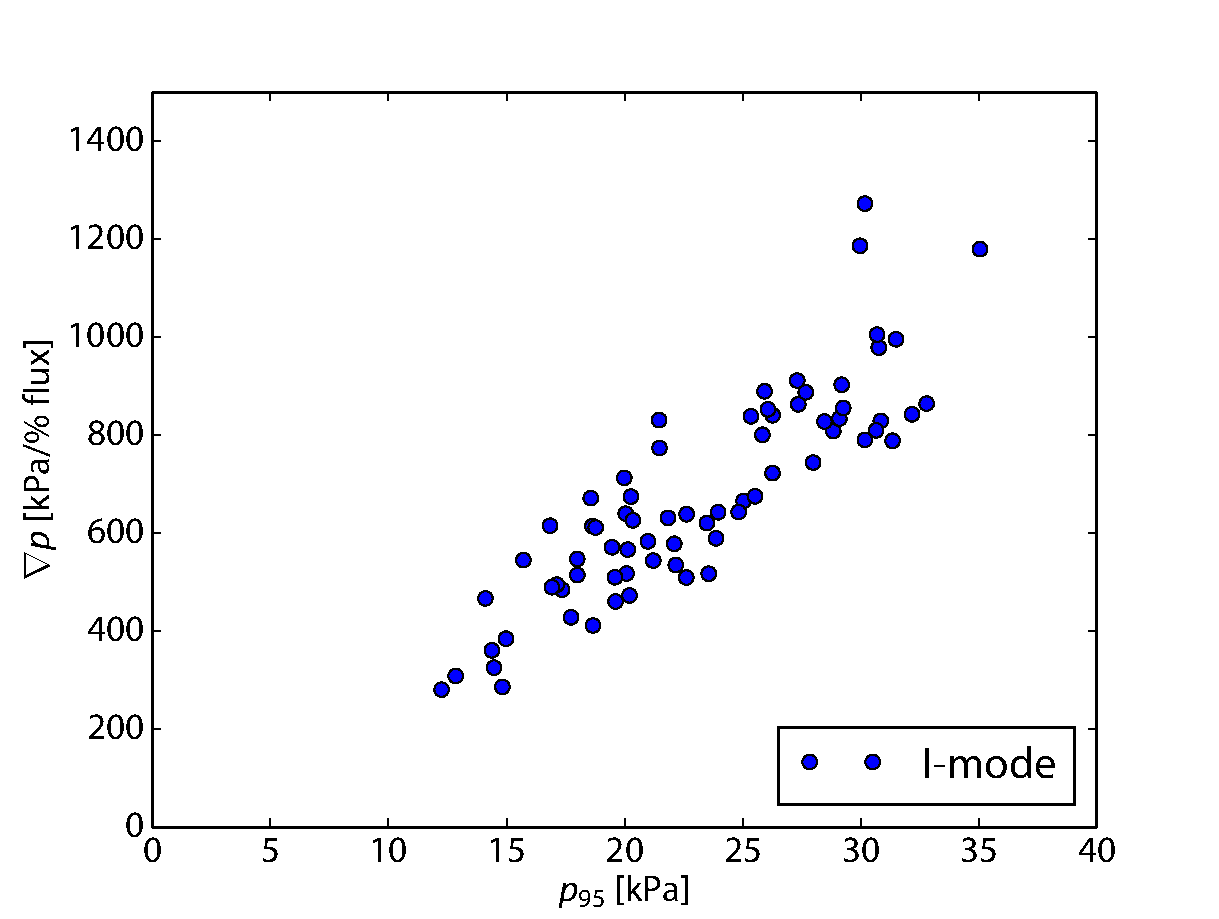
\includegraphics[width=100mm]{graphics/IModePedestal/p95_gradp_i.pdf}}
\end{figure}

In \cref{subsec:imode_kbm,subsec:imode_exp_widths}, the I-mode pedestal width (both in temperature and pressure) is shown to be insensitive to a number of pedestal parameters.  This may be examined directly by viewing the peak pedestal gradient versus its height -- to lowest approximation, $\nabla Y \sim Y/\Delta_Y$ (where $Y$ is the pedestal quantity, \ie $T_e$, $p_{tot}$).  The peak gradients in temperature and pressure are shown against the corresponding 95\%-flux values in \cref{fig:imode_Te_gradT} and \cref{fig:imode_p_gradp}, respectively.  In both cases, a linear dependence of the gradient on the pedestal-top value is observed, albeit with scatter favoring higher gradients than the linear prediction in the case of the temperature.  The pressure gradient is predicted quite well by its 95\%-flux value.  Similar behavior has been observed for the electron and ion temperatures in H-mode on AUG and DIII-D, independent of plasma shaping and evidently operating under a separate limit from the ideal-MHD constraint on the pressure pedestal \cite{Schneider2013}.  These trends are consistent with robust pedestal widths, particularly in the pressure pedestal, in I-mode.\nicesectionending

\section{Global Behavior, Performance, \& Confinement}\label{sec:imode_confinement}

The pedestal structure of the I-mode is quite desirable for a reactor scenario -- due to the strong response of the pedestal temperature to heating power, externally-applied heating power is an effective engineering control for core temperatures, and subsequently fusion reaction rates.  The high pedestal temperature, coupled to stiff core temperature profiles (such that a higher temperature supports a steeper marginally-stable $\nabla T_e$)\gnote{worth showing core $T_e$ profile behavior, \ie bulk calculation of $R/L_{T_e}$?}, supports very high core temperatures.  With a moderate degree of core density peaking\gnote{Working on density peaking calculations in I-mode, should go fairly quickly}, this supports comparable core and volume-averaged pressures to H-mode despite the comparatively relaxed pedestal, supporting beneficial fusion conditions in the core while avoiding stability issues in the pedestal.  Example density, temperature, and pressure profiles for I-mode and H-mode cases are shown in \cref{fig:imode_coreprofs}, illustrating the high core pressures attainable in I-mode despite the lower pedestal and reduced density.  This is reflected in \cref{fig:imode_betan_H}, showing the global-averaged normalized beta ($\langle \beta_N \rangle = \langle \beta \rangle a B_T/I_p$) versus the confinement metric $H_{98}$ in I-mode and ELMy H-mode -- I-mode reaches comparable levels of $\beta_N$ while maintaining H-mode-like $H_{98} \sim 1$ at comparable levels to ELMy H-mode, while maintaining desirable impurity confinement and ELM stability behaviors.

\begin{figure}[p]
 \pushtooutside
 \fcapside[60mm]{\caption[Density, temperature, and pressure profiles in I-mode and EDA H-mode.]{Profiles in density, temperature, and pressure for I-mode and EDA H-mode.  The H-mode case exhibits a very strong density pedestal, with a somewhat reduced temperature pedestal; the I-mode, in contrast, has a significant temperature pedestal with a relaxed density profile.  While this typically results in a reduced pedestal pressure in I-mode compared to H-mode, core profile stiffness supports very high central temperatures, such that I-mode exhibits comparable core and average pressure despite the reduced pedestal.}\label{fig:imode_coreprofs}}{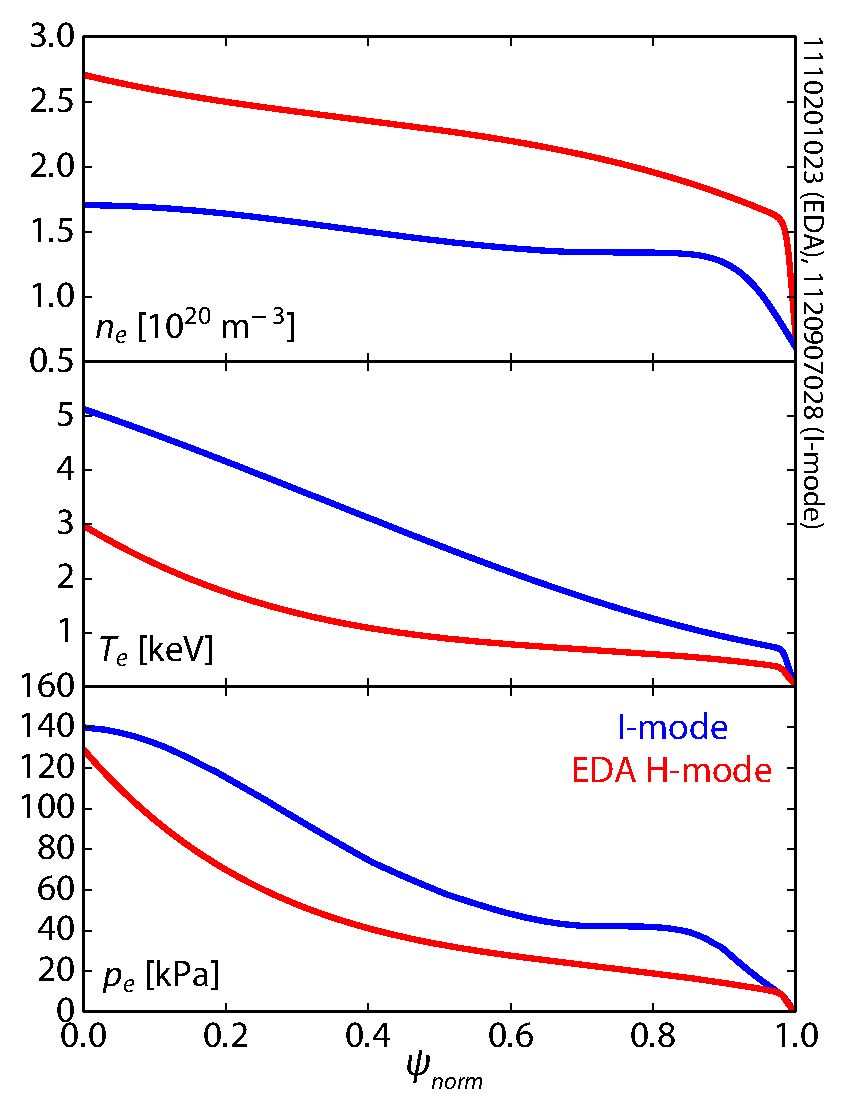
\includegraphics[width=100mm]{graphics/IModePedestal/coreprof.pdf}}
\end{figure}

\begin{figure}[p]
 \pushtooutside
 \fcapside[60mm]{\caption[Normalized beta vs. $H_{98}$ for I-mode and ELMy H-mode.]{Global normalized $\beta_N$ versus confinement factor $H_{98}$ for I-mode and ELMy H-mode.  Despite the relaxed pedestal pressure, I-modes reach comparable average pressures, while maintaining H-mode-like energy confinement.}\label{fig:imode_betan_H}}{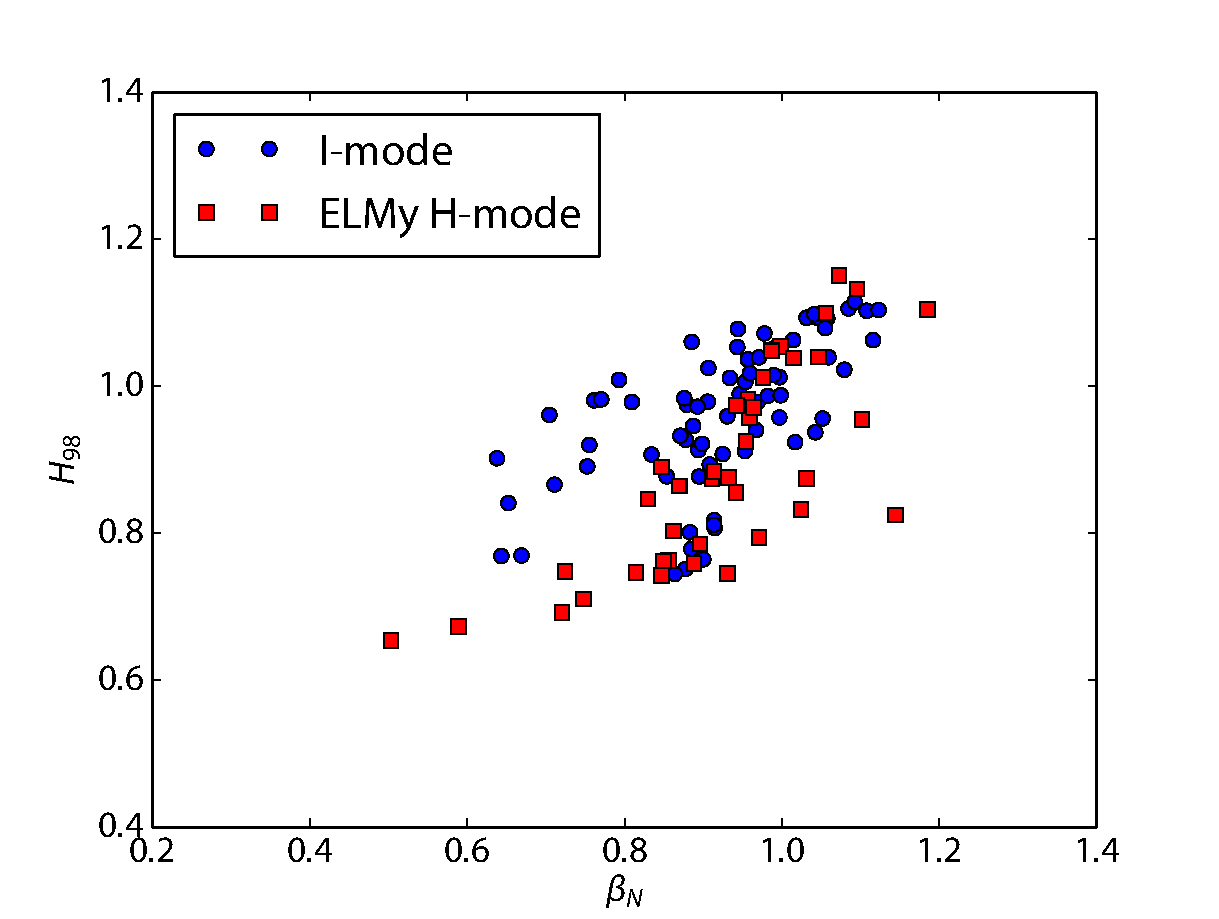
\includegraphics[width=100mm]{graphics/IModePedestal/betan_H_i_e.pdf}}
\end{figure}

\begin{figure}[p]
 \pushtooutside
 \fcapside[60mm]{\caption[I-mode stored energy vs. heating power times plasma current.]{I-mode stored energy versus the product of net heating power $P_{net}$ and plasma current $I_p$.  Based on the H-mode confinement scaling, $\tau_E$ is expected to scale linearly with $I_p$, and to show a strong degradation with heating power: $\tau_E \sim I_p \times P_{net}^{-0.7}$.  As the stored energy is given by $W \sim P_{net} \tau_E$, $W \sim I_p P_{net}^{0.3}$ is expected.  The observed linear trend indicates little-to-no degradation of $\tau_E$ in I-mode with heating power.}\label{fig:imode_PIp_W}}{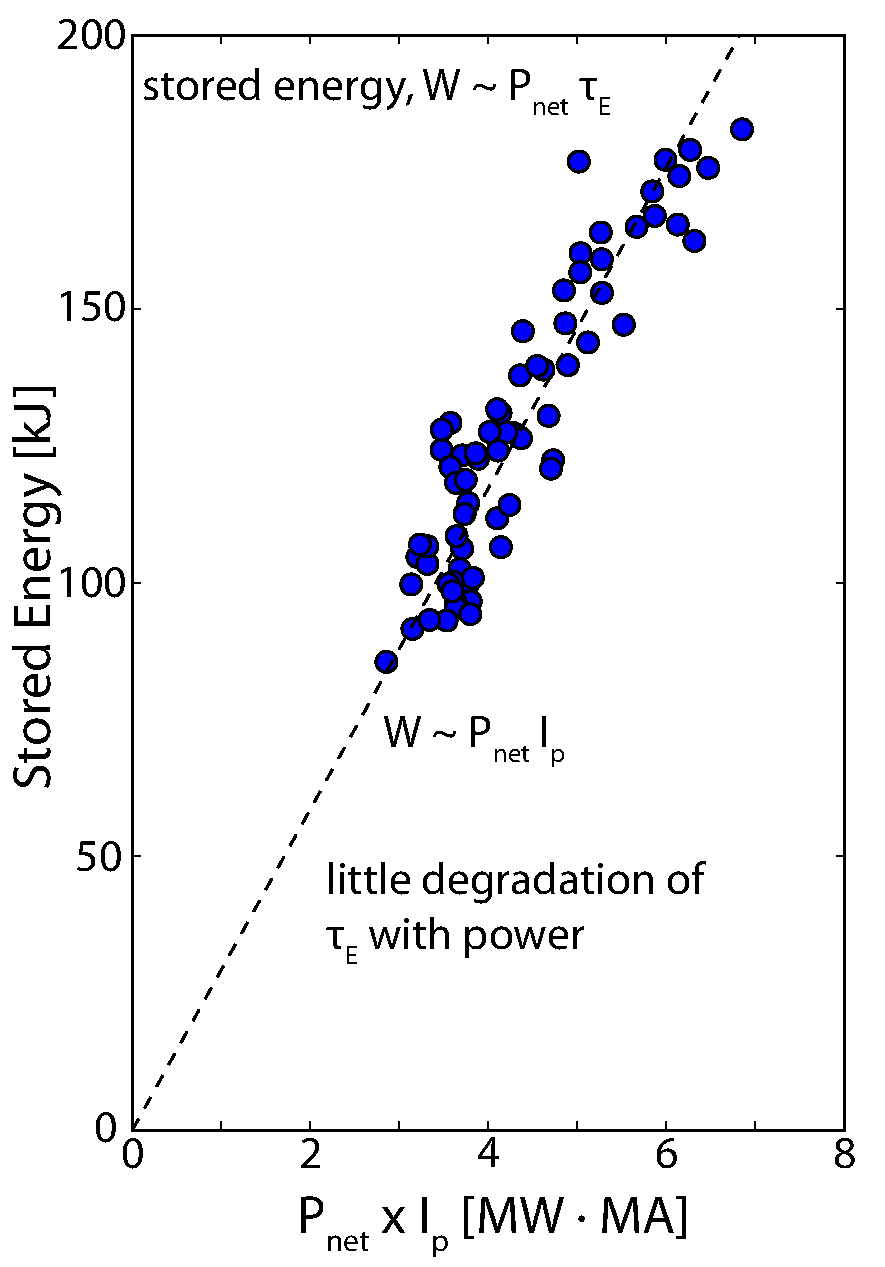
\includegraphics[width=100mm]{graphics/IModePedestal/PIp_W_scale.pdf}}
\end{figure}

\begin{figure}[p]
 \pushtooutside
 \fcapside[60mm]{\caption[Stored energy versus fueling in I-mode and H-mode.]{Plasma stored energy versus fueling, indicated by $\overline{n}_e$ in I-mode and ELMy H-mode.  I-mode stored energy increases strongly with fueling (provided sufficient power to maintain the temperature pedestal), while ELMy H-mode exhibits little trend with density -- the global stored energy and average pressure is set by the pedestal beta, which is strongly limited in ELMy H-mode.}\label{fig:imode_nebar_W}}{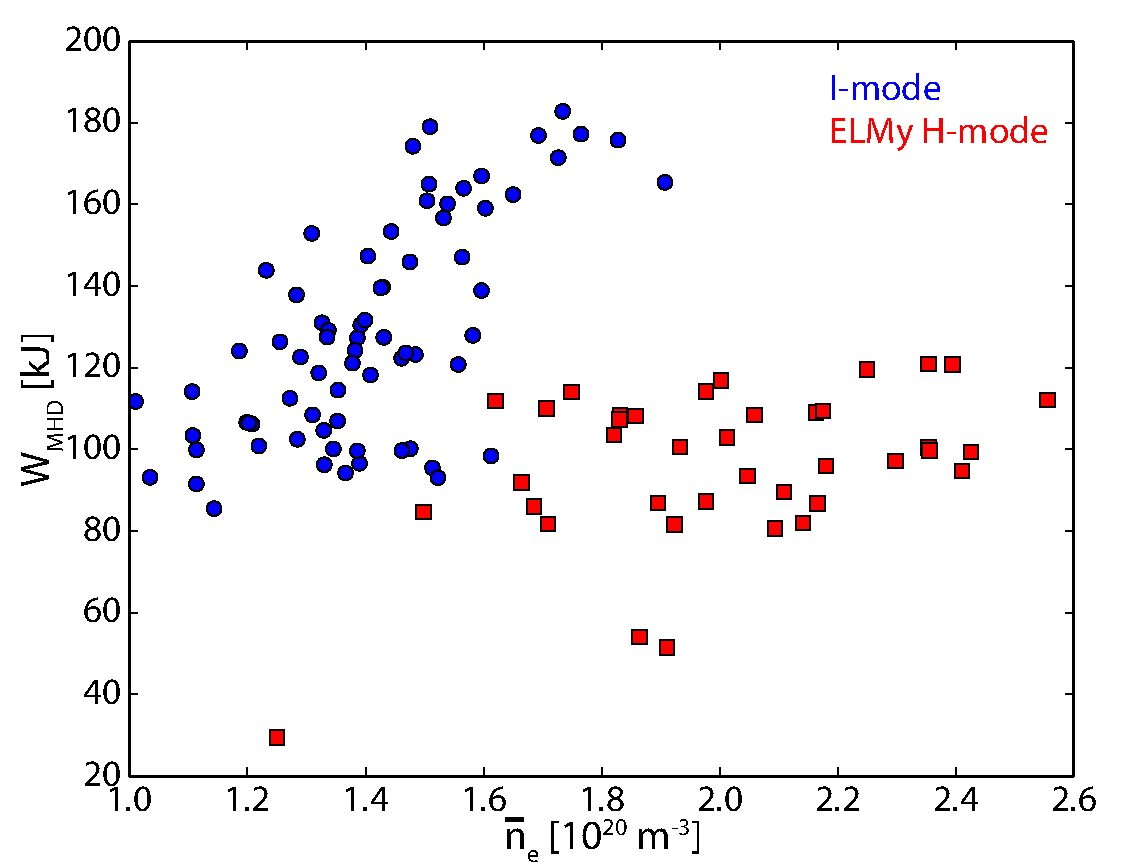
\includegraphics[width=100mm]{graphics/IModePedestal/nebar_W_i_e.pdf}}
\end{figure}

Energy confinement in I-mode also appears to lack strong degradation with heating power (\cf the $\tau_E \sim P^{-0.7}$ degradation for H-modes, as in \cref{eq:tau98}) -- a highly desirable characteristic for large devices.  This may be seen intuitively in \cref{fig:imode_PIp_W}.  The plasma stored energy trends as $W \sim P \tau_E$; from the H-mode scaling, we expect $\tau_E \sim I_p$.  The H-mode confinement scaling, then, predicts $W \sim I_p P_{net}^{0.3}$.  However, the stored energy in I-mode trends as $W \sim P_{net} I_p$, indicating that there is little or no (negative) dependence of $\tau_E$ on heating power in I-mode.  The strong dependence of the stored energy on heating power is reflected in the response of the pressure pedestal to the same, shown in \cref{fig:imode_Pnet_p95}.  The degradation of energy confinement with heating power in H-mode reflects the MHD limits on the pedestal -- increased heating power raises the ELM frequency to drive enhanced energy transport, maintaining the pedestal at the MHD limit, which in turn drives the weak increase of stored energy with increased power.  The lack of power degradation in I-mode, then, reflects the stability of the pedestal against ELMs.

Similarly, the beneficial response to fueling in the I-mode pedestal is reflected in global confinement, as the stored energy increases strongly with fueling levels (\cref{fig:imode_nebar_W}).    In contrast, ELMy H-mode stored energy is largely insensitive to fueling.  The stored energy and core $\beta_N$ is instead set by the pedestal beta, which is set predominantly by plasma shape (note, however, that there is a non-negligible effect of density vs. temperature on the core pressure, with hotter, lower-density pedestals leading to higher core pressures due to stiff temperature profiles -- however, these lower-collisionality pedestals tend to exhibit larger ELMs as well).

\subsection{Confinement Scaling Laws}\label{subsec:imode_powerlaws}

Due to the complexity inherent in modeling global energy transport from first-principles physics, it is common to establish empirical scaling laws for energy confinement using a power-law fit to large datasets.  For example, the ITER89 \cite{Yushmanov1990} and ITER98 \cite{ITER1999} scalings utilized an extensive multi-machine database \cite{Christiansen1992} for L-mode and H-mode confinement.  In particular the ITER98y2 scaling (see \cref{eq:tau98}) is a commonly-used baseline for high-performance regimes, particularly in terms of the normalized $H_{98}$ (\cref{eq:H98}).  However, as the ITER98y2 scaling was constructed predominantly with type-I ELMy H-modes (as these customarily are the highest-performance H-modes on most tokamaks), and as such implicitly includes the physics of ELM-limited pedestals.  For example, the power-law fit in ITER98y2 includes a strong degradation of confinement with heating power, $\tau_E \sim P^{-0.7}$.  This is consistent with the observed weak response of ELMing pedestals with heating power \cite{Snyder2007}, with increased power instead raising the ELM frequency to maintain consistent ELM-driven heat transport.

In light of the substantially different physics of the I-mode pedestal and energy confinement compared to H-modes, it is useful to construct a power-law confinement fit using I-mode data.  It is strongly emphasized that such a fit would be only preliminary, as fits using data from a single machine lack the range of parameter values needed to extrapolate to larger devices.  I-mode energy confinement times are fitted in a least-squares sense to the general form

\begin{equation}\label{eq:taufit}
 \tau_{I-mode} = C \; I_p^{\alpha_{I_p}} \; B_T^{\alpha_{B_T}} \; \overline{n}_e^{\alpha_{n_e}} \; R^{\alpha_R} \; \varepsilon^{\alpha_\varepsilon} \; \kappa^{\alpha_\kappa} \; P_{loss}^{\alpha_P}
\end{equation}

\noindent to find free exponents $\alpha_j$ for plasma current $I_p$ in $\si{\mega\ampere}$, toroidal field $B_T$ in $\si{\tesla}$, line-averaged density $\overline{n}_e$ in $\SI{e20}{\per\meter\cubed}$, major radius $R$ in $\si{\meter}$, inverse aspect ratio $\varepsilon$, elongation $\kappa$, and loss power $P_{loss}$ in $\si{\mega\watt}$ (see \cref{eq:ploss}).  To extend the quantity of data and range of parameters available for this assay, the high-resolution pedestal data used in the bulk of this thesis is supplemented by older I-mode datasets containing both reversed-field LSN and forward-field USN I-mode cases.  Although these data lack the high-resolution edge data necessary for pedestal structure and stability studies, they are nevertheless suitable for scalings based on global parameters.  Although the net power $P_{net}$ (see \cref{eq:pnet}) has been demonstrated to be the more suitable parameter, rather than $P_{loss}$ \cite{Hughes2002}, these older data contain inconsistent measurements of the radiated power, necessitating the use of loss power in its stead.  However, the radiated power is typically a fairly small fraction of the total power in I-mode ($P_{rad} < \SI{900}{\kilo\watt}$, $P_{rad}/P_{tot} < 20\%$), and in any case this is consistent with previous confinement scaling studies, so the use of $P_{loss}$ is sufficient for a first-pass examination of confinement.

\begin{table*}
 \pushtooutside
 \ttabbox{\caption[Parameters for power-law scalings of I-mode energy confinement time.]{Parameters for power-law scalings of the I-mode energy confinement time $\tau_E$, along with $R^2$ coefficients of determination for the fit.  Blank entries indicate parameters that were omitted from that fit.  Note that fit \#5 utilized a fixed $R^2 \sqrt{\varepsilon}$ size dependence rather than taking the size to be a free fitting parameter.  Parameters are in the given units: $I_p$ in $\si{\mega\ampere}$, $B_T$ in $\si{\tesla}$, $\overline{n}_e$ in $\SI{e20}{\per\meter\cubed}$, $R$ in $\si{\meter}$, and $P_{loss}$ in $\si{\mega\watt}$.  Elongation $\kappa$ and aspect ratio $\varepsilon$ are dimensionless.}\label{tab:imode_confinement}}{
 \begin{tabular}{cccccc}
  \toprule
  & \#1 & \#2 & \#3 & \#4 & \#5 \\
  \midrule
  $C$ & $0.040 \pm 0.066$ & $0.007 \pm 0.002$ & $0.014 \pm 0.002$ & $0.014 \pm 0.002$ & $0.056 \pm 0.008$ \\
  $I_p$ & $0.686 \pm 0.074$ & $0.696 \pm 0.073$ & $0.685 \pm 0.076$ & $0.692 \pm 0.073$ & $0.676 \pm 0.077$ \\
  $B_T$ & $0.698 \pm 0.075$ & $0.697 \pm 0.071$ & $0.768 \pm 0.072$ & $0.773 \pm 0.071$ & $0.767 \pm 0.072$ \\
  $\overline{n}_e$ & $-0.077 \pm 0.055$ & $-0.050 \pm 0.048$ & $0.017 \pm 0.048$ & & $0.006 \pm 0.048$ \\
  $R$ & $4.219 \pm 4.623$ & & & & $2^*$ \\
  $\varepsilon$ & $0.127 \pm 1.144$ & & & & $0.5^*$ \\
  $\kappa$ & $1.686 \pm 0.398$ & $1.501 \pm 0.350$ & & & \\
  $P_{loss}$ & $-0.197 \pm 0.048$ & $-0.220 \pm 0.043$ & $-0.286 \pm 0.042$ & $-0.281 \pm 0.039$ & $-0.275 \pm 0.042$ \\
  $R^2$ & $0.713$ & $0.711$ & $0.685$ & $0.684$ & $0.683$ \\
  \bottomrule
 \end{tabular}
 }
\end{table*}

Results from a number of scaling studies are shown in \cref{tab:imode_confinement}, containing the values and standard deviations for each exponent value, the scale factor $C$, and the $R^2$ coefficient of determination.  We begin with the full parameter list used in the ITER98y2 scaling, shown as fit \#1 in \cref{tab:imode_confinement}, with results shown in \cref{fig:imode_tauE_1}.  However, it is immediately obvious that the size scalings, dependent on major radius $R$ and inverse aspect ratio $\varepsilon$, are not properly captured (denoted by the extreme errorbars on these parameters).  This is to be expected -- absent meaningful variation in $R$ and $\varepsilon$ in the dataset (which requires multiple machines to produce) these parameters are not well-constrained, and result \#1 is over-fitted.  

For simplicity, we reduce our consideration to an effective single-machine scaling, omitting these parameters (indicated by blank entries in \cref{tab:imode_confinement}).  Under this fit, shown as \#2 in \cref{tab:imode_confinement}, the power applied to the elongation $\kappa$ is elevated compared to that expected from the ITER98y2 scaling, with the relatively large deviation expected from the somewhat restricted range of shapes found in these studies.  Omitting this fitting parameter results a minimum-complexity fit,

\begin{equation}\label{eq:tauE_fit_3}
 \tau_{I-mode} = 0.014 \times I_p^{0.685} \; B_T^{0.768} \; \overline{n}_e^{0.017} \; P_{loss}^{-0.286}
\end{equation}

\noindent with a coefficient of determination of $R^2 = 0.685$ (also shown as \#3 in \cref{tab:imode_confinement}).  The correspondence between experimenal $\tau_E$ and the modeled confinement time is shown in \cref{fig:imode_tauE_3}.  The density dependence in $\tau_E$ is quite weak, and may be omitted (fit \#4) with minimal alteration to the result; however, this may not capture effects on the transport at higher Greenwald fraction, and requires additional experiments.

\begin{figure}[t]
 \pushtooutside
 \begin{floatrow}
  \ffigbox[\FBwidth]{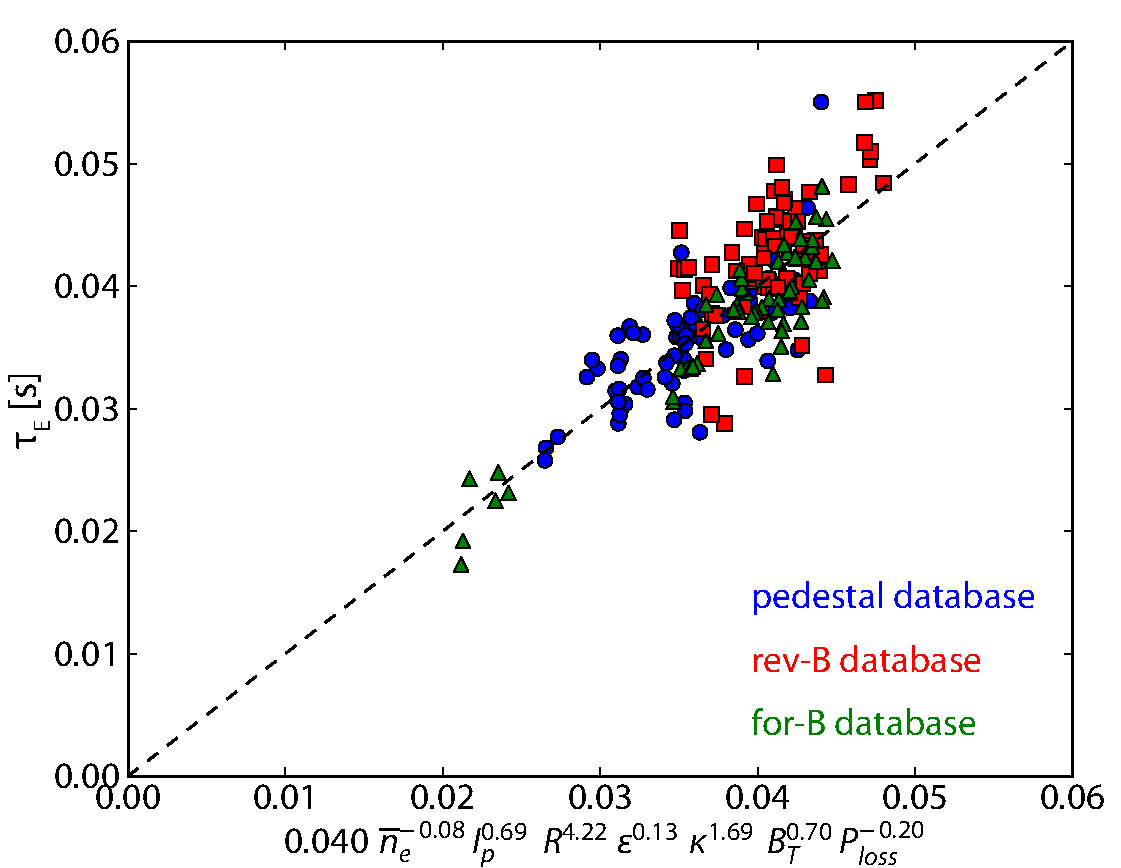
\includegraphics[width=75mm]{graphics/IModePedestal/tauE_1_Ploss_sep.pdf}}{\caption[Power-law fit to I-mode $\tau_E$ with full parameter set.]{Power-law fit for I-mode energy confinement time $\tau_E$, fitted using the full ITER98y2 parameter set (fit \#1 in \cref{tab:imode_confinement}).  Both the high-resolution pedestal database and older reversed-field LSN and forward-field USN I-mode databases are used.  While the fit is generally good, lack of variation in certain parameters -- particularly the size parameters $R$ and $\varepsilon$ (as expected for a single-machine scaling), and elongation $\kappa$ mean that the true variation with these parameters is not accurately captured.  However, the expected weak degradation of $\tau_E$ with heating power is captured.}\label{fig:imode_tauE_1}}
  \ffigbox[\FBwidth]{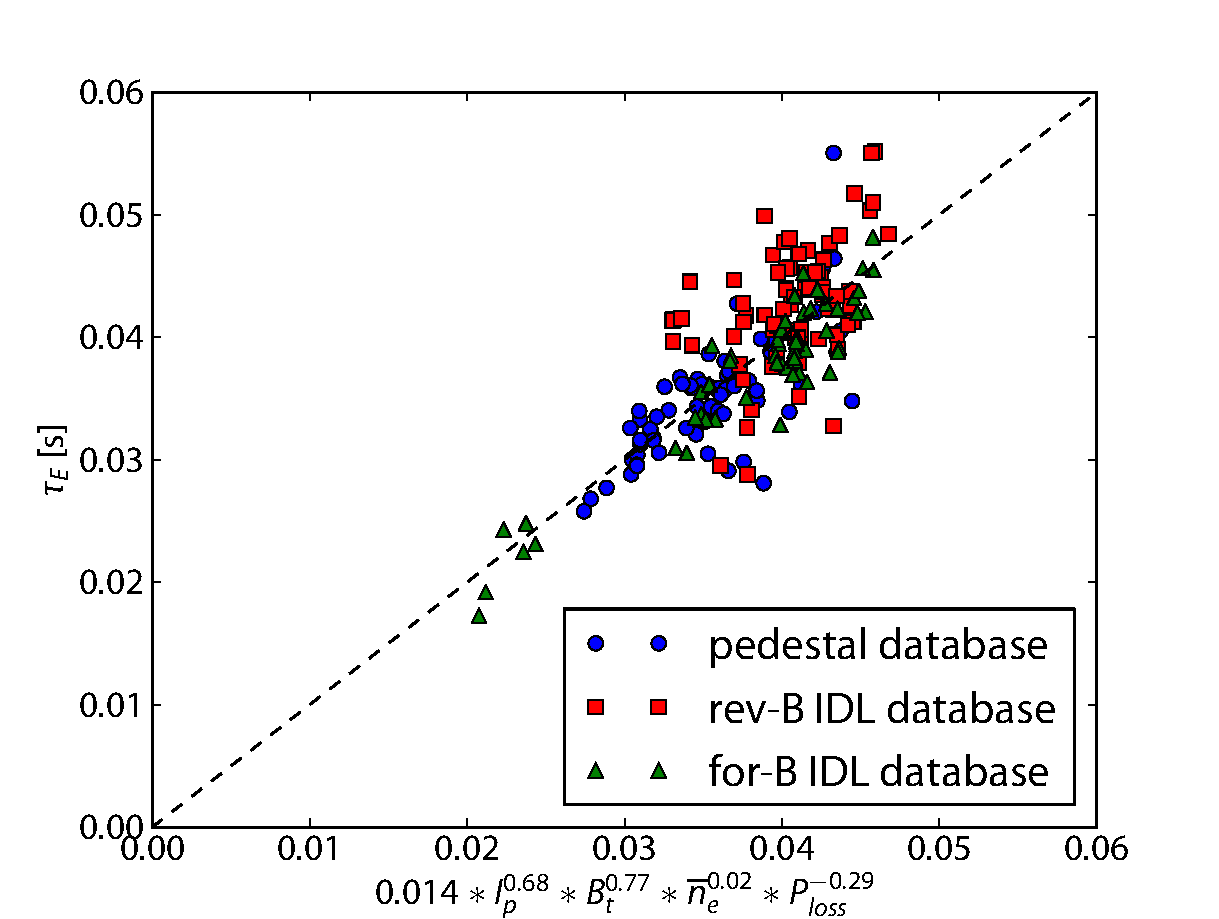
\includegraphics[width=75mm]{graphics/IModePedestal/tauE_3_Ploss_sep.pdf}}{\caption[Power-law fit to I-mode $\tau_E$, with poorly-fitted parameters excluded.]{Power-law fit for I-mode energy confinement time $\tau_E$, fitted with the size parameters $R$ and $\varepsilon$, and elongation $\kappa$ excluded due to the lack of variation in these variables in the available data (fit \#3 in \cref{tab:imode_confinement}).  Both the high-resolution pedestal database and older reversed-field LSN and forward-field USN I-mode databases are used.  This represents the minimum-complexity fit for I-modes on C-Mod, capturing the essential dependences on current, field, and fueling, and notably the weak degradation of confinement with heating power.}\label{fig:imode_tauE_3}}
 \end{floatrow}
\end{figure}

\begin{figure}[t]
 \pushtooutside
 \begin{floatrow}
  \ffigbox[\FBwidth]{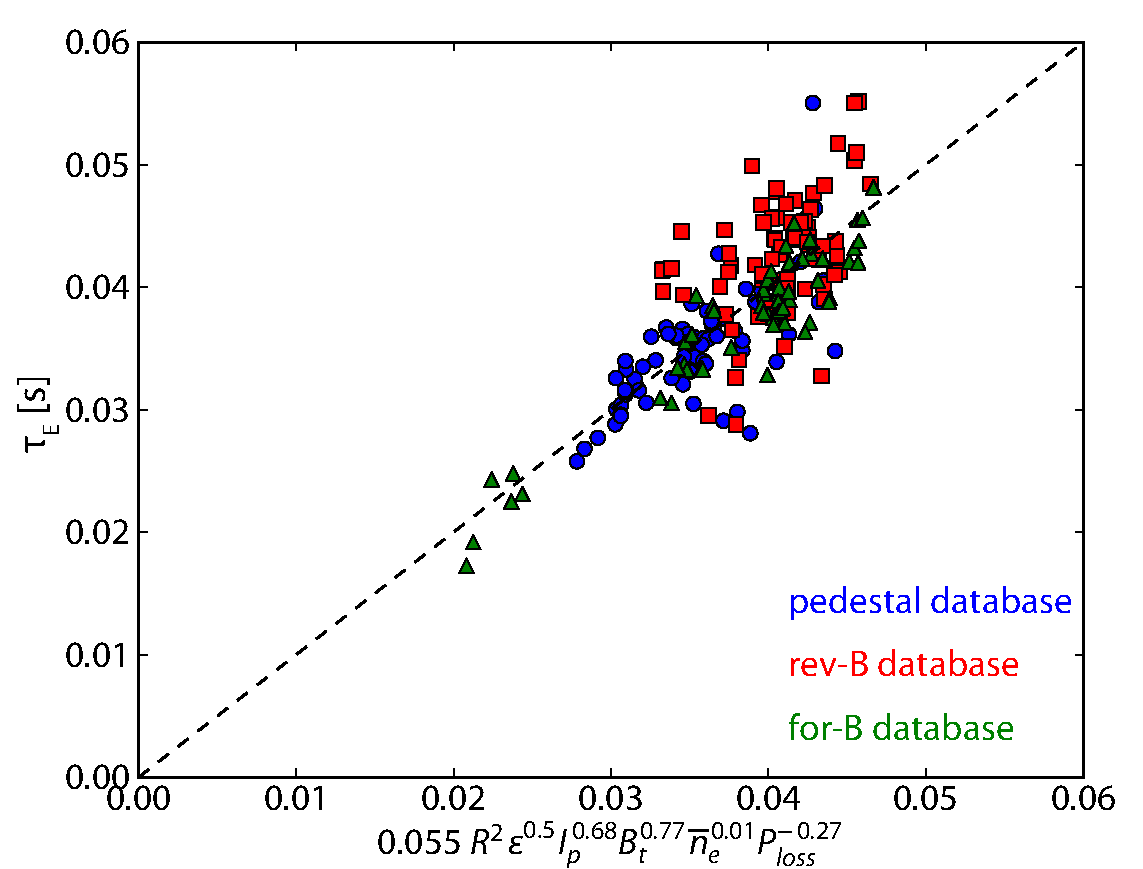
\includegraphics[width=75mm]{graphics/IModePedestal/tauE_6_Ploss_sep.pdf}}{\caption[Power-law fit to I-mode $\tau_E$, with fixed $R^2 \sqrt{\varepsilon}$ size scaling.]{Power-law fit to I-mode energy confinement time $\tau_E$, with the \emph{ansatz} of an $R^2 \sqrt{\varepsilon}$ size scaling fixed (fit \#5 in \cref{tab:imode_confinement}).  Both the high-resolution pedestal database and older reversed-field LSN and forward-field USN I-mode databases are used.  Note the expected weak degradation of $\tau_E$ with heating power.}\label{fig:imode_tauE_6}}
  \ffigbox[\FBwidth]{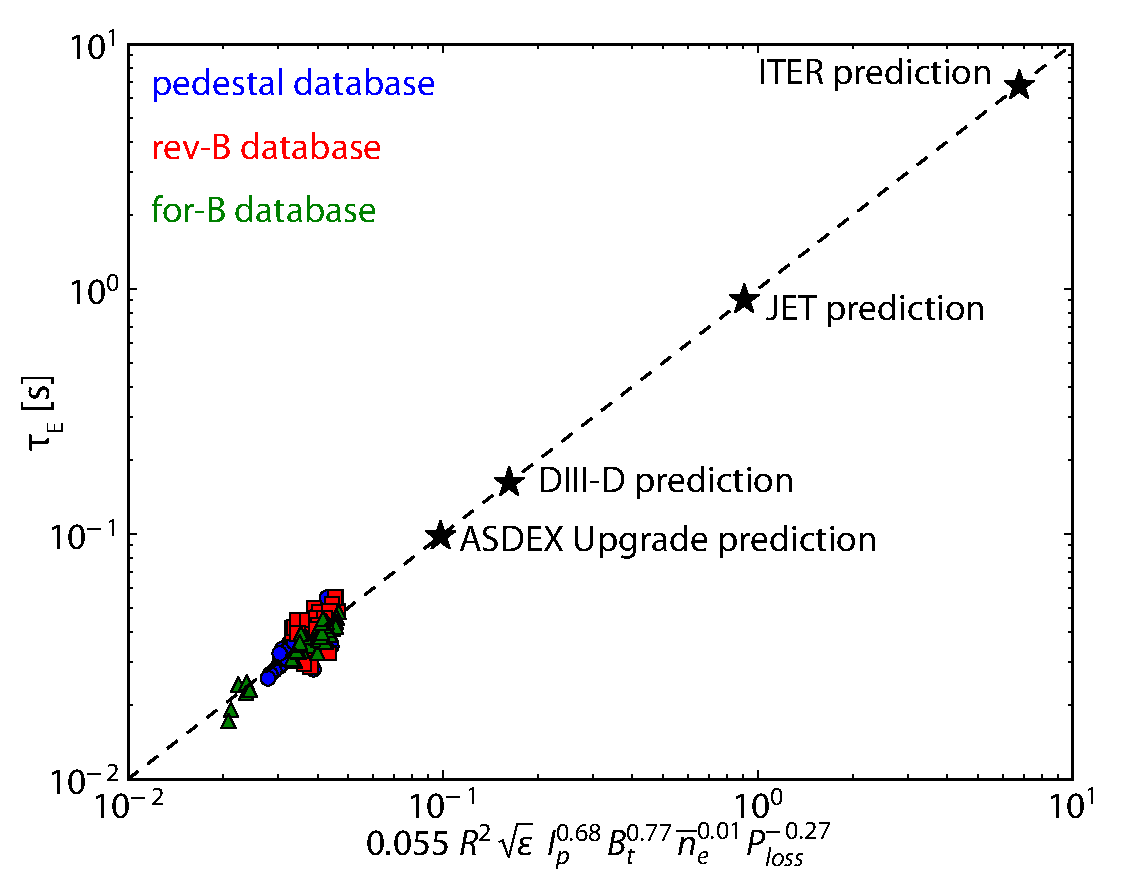
\includegraphics[width=75mm]{graphics/IModePedestal/tauE_6_Ploss_extrap.pdf}}{\caption[Power-law fit to I-mode $\tau_E$ extrapolated to larger devices.]{Modeled energy confinement time $\tau_E$ with the fixed $R^2 \sqrt{\varepsilon}$ size scaling (fit \#5 in \cref{tab:imode_confinement}, extrapolated to DIII-D, ASDEX Upgrade, JET, and ITER.  Modeled energy confinement times are competitive with H-modes, both the measured $\tau_E$ for existing machines and the expected ITER98y2 prediction for ITER H-modes.}\label{fig:imode_tauE_extrap}}
 \end{floatrow}
\end{figure}

As an illustrative exercise, we restore a fixed size dependence of the form $R^2 \sqrt{\varepsilon}$ (as is found in ITER98y2) to the fit, shown as \#5 in \cref{tab:imode_confinement}, with the correspondence to experimental $\tau_E$ shown in \cref{fig:imode_tauE_6}.  This enables extrapolation of the result to larger devices, with example predictions for DIII-D, ASDEX Upgrade, JET, and ITER shown in \cref{fig:imode_tauE_extrap}.  Due to the weakened power degradation ($\tau_E \sim P^{-0.2}$), I-mode operation on ITER (in the putative $Q=10$ scenario with $\SI{100}{\mega\watt}$ of alpha heating) projects to a $\sim \SI{8}{\second}$ energy confinement time, well in excess of the expected $\tau_E$ for H-mode.

Again, we emphasize that single-machine scalings are of limited reliability for extrapolative purposes.  However, this illustrates the potential gains in performance in the application of I-mode to larger devices, while correctly capturing the observed physics in I-mode (\eg the degradation in $\tau_E$ is, to within uncertainty, consistent with the observed strong dependence of the stored energy and pedestal pressure on heating power).  However, it is notable that preliminary results in I-mode experiments on ASDEX Upgrade\gnote{must clear this with F. Reiter!} observed energy confinement times in the range of $0.07-\SI{0.1}{\second}$, consistent with the predictions of the I-mode model in the corresponding parameter range, although detailed analysis of these shots has not been performed.\nicesectionending

%\begin{figure}
% \pushtooutside
% \fcapside[60mm]{\caption[Power-law fit to I-mode $\tau_E$ with full parameter set.]{Power-law fit for I-mode energy confinement time $\tau_E$, fitted using the full ITER98y2 parameter set (fit \#1 in \cref{tab:imode_confinement}).  Both the high-resolution pedestal database and older reversed-field LSN and forward-field USN I-mode databases are used.  While the fit is generally good, lack of variation in certain parameters -- particularly the size parameters $R$ and $\varepsilon$ (as expected for a single-machine scaling), and elongation $\kappa$ mean that the true variation with these parameters is not accurately captured.  However, the expected weak degradation of $\tau_E$ with heating power is captured.}\label{fig:imode_tauE_1}}{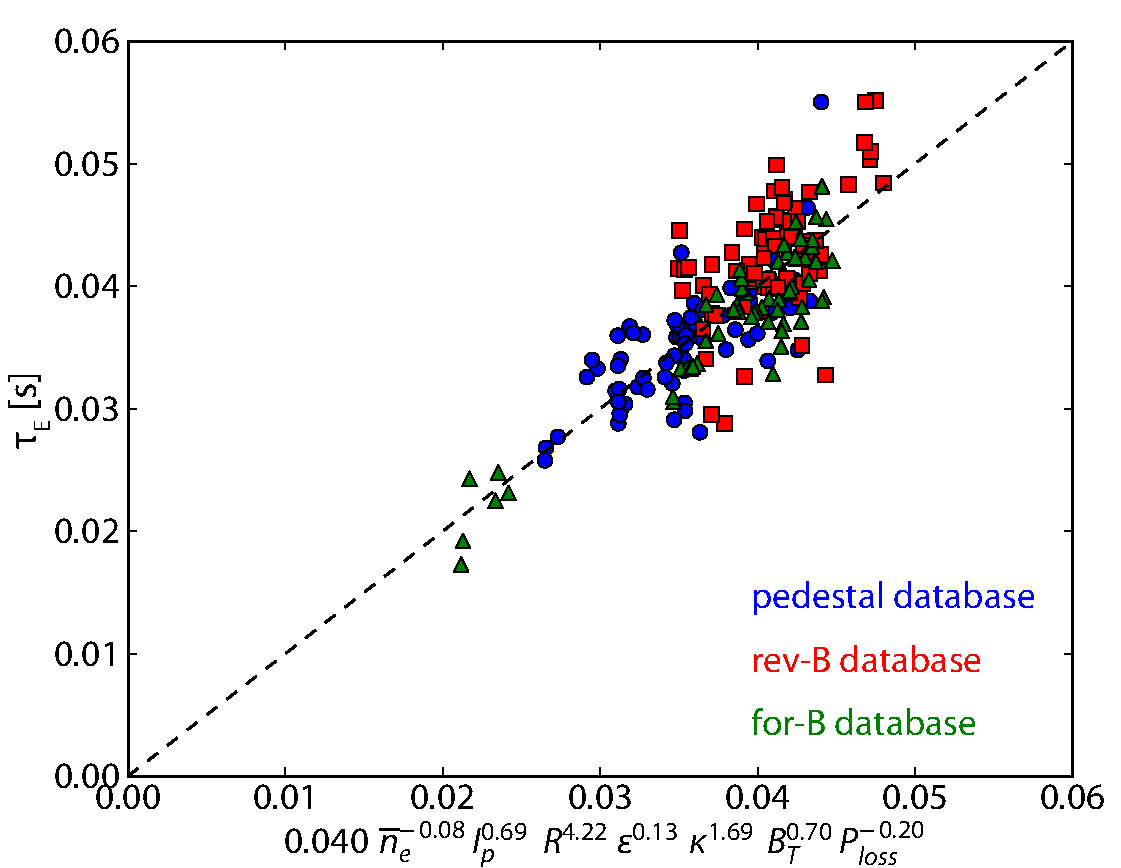
\includegraphics[width=100mm]{graphics/IModePedestal/tauE_1_Ploss_sep.pdf}}
%\end{figure}

%\begin{figure}
% \pushtooutside
% \fcapside[60mm]{\caption[Power-law fit to I-mode $\tau_E$, with poorly-fitted parameters excluded.]{Power-law fit for I-mode energy confinement time $\tau_E$, fitted with the size parameters $R$ and $\varepsilon$, and elongation $\kappa$ excluded due to the lack of variation in these variables in the available data (fit \#3 in \cref{tab:imode_confinement}).  Both the high-resolution pedestal database and older reversed-field LSN and forward-field USN I-mode databases are used.}\label{fig:imode_tauE_3}}{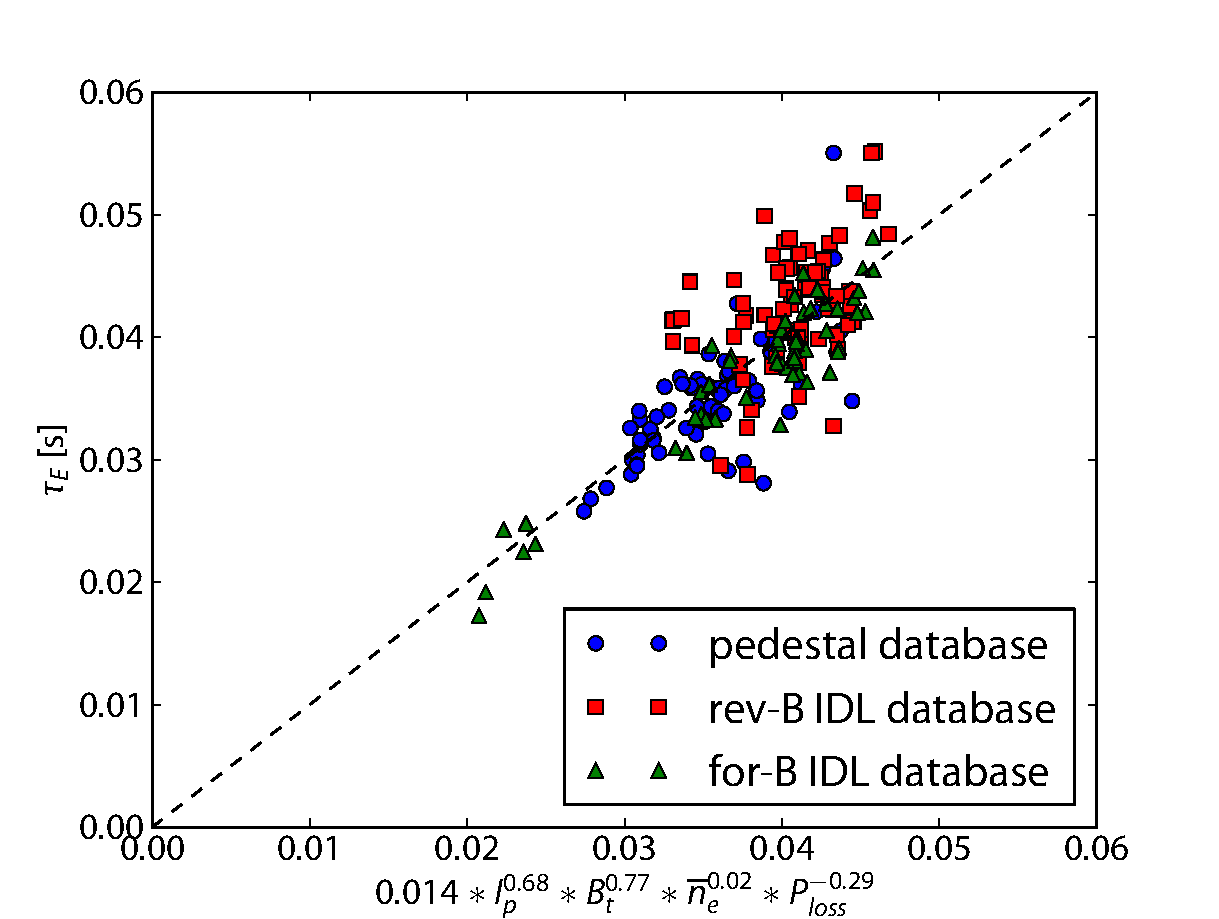
\includegraphics[width=100mm]{graphics/IModePedestal/tauE_3_Ploss_sep.pdf}}
%\end{figure}

%\begin{figure}
% \pushtooutside
% \fcapside[60mm]{\caption[Power-law fit to I-mode $\tau_E$, with fixed $R^2 \sqrt{\varepsilon}$ size scaling.]{Power-law fit to I-mode energy confinement time $\tau_E$, with the \emph{ansatz} of an $R^2 \sqrt{\varepsilon}$ size scaling fixed (fit \#5 in \cref{tab:imode_confinement}).  Both the high-resolution pedestal database and older reversed-field LSN and forward-field USN I-mode databases are used.  Note the expected weak degradation of $\tau_E$ with heating power.}\label{fig:imode_tauE_6}}{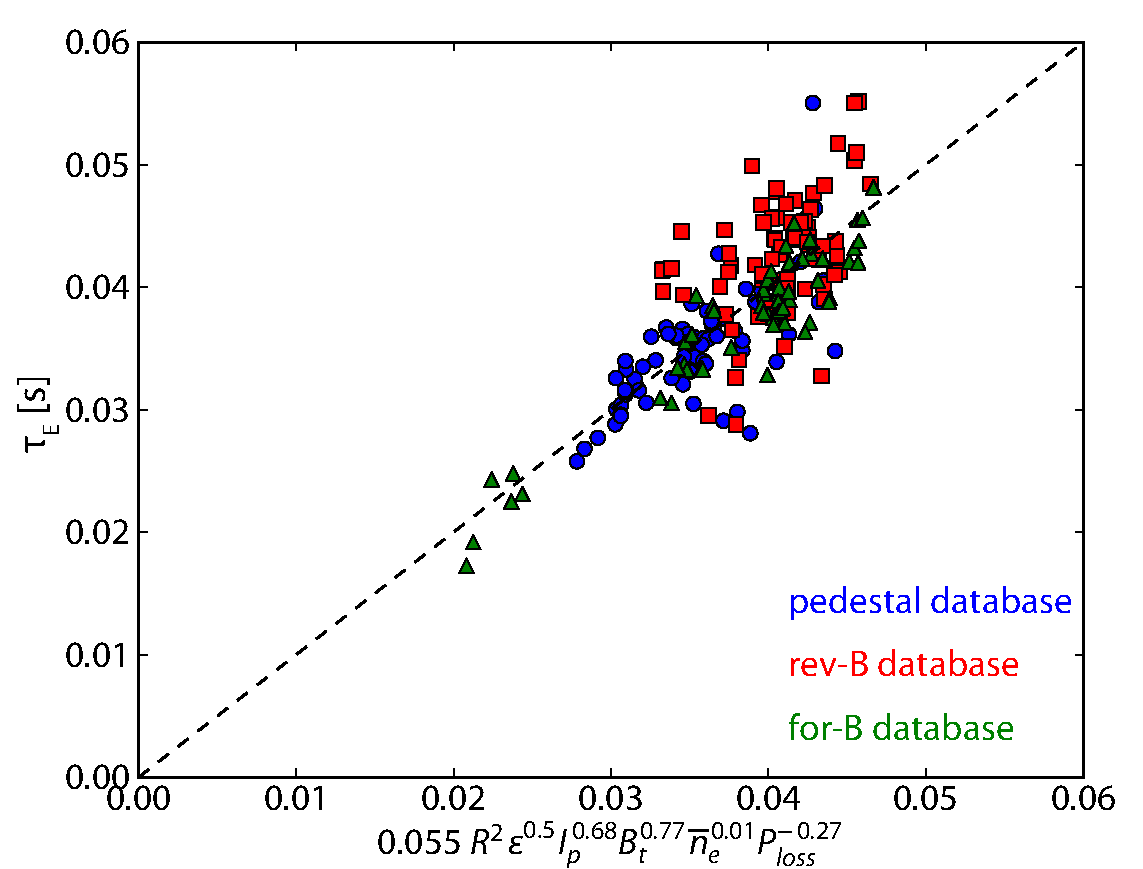
\includegraphics[width=100mm]{graphics/IModePedestal/tauE_6_Ploss_sep.pdf}}
%\end{figure}
%
%\begin{figure}
% \pushtooutside
% \fcapside[60mm]{\caption[Power-law fit to I-mode $\tau_E$ extrapolated to larger devices.]{Modeled energy confinement time $\tau_E$ with the fixed $R^2 \sqrt{\varepsilon}$ size scaling (fit \#5 in \cref{tab:imode_confinement}, extrapolated to DIII-D, ASDEX Upgrade, JET, and ITER.  Modeled energy confinement times are competitive with H-modes, both the measured $\tau_E$ for existing machines and the expected ITER98y2 prediction for ITER H-modes.}\label{fig:imode_tauE_extrap}}{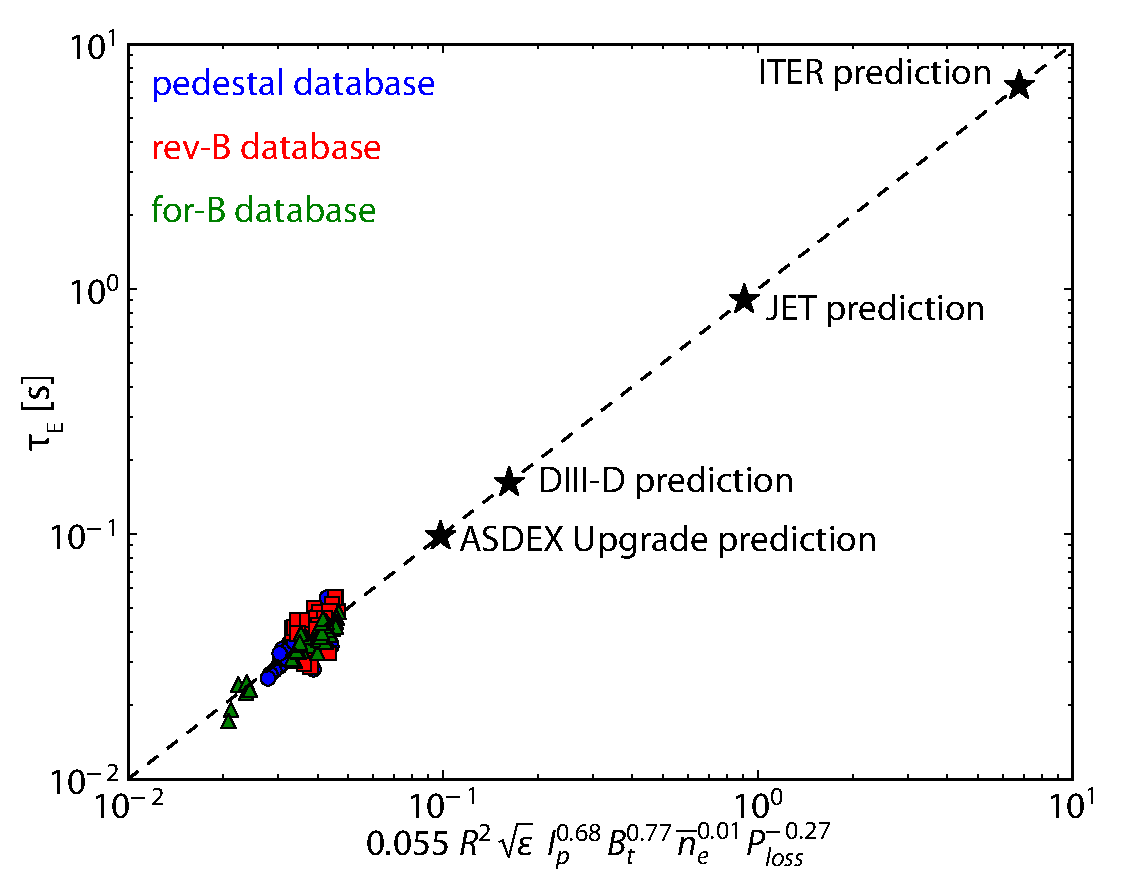
\includegraphics[width=100mm]{graphics/IModePedestal/tauE_6_Ploss_extrap.pdf}}
%\end{figure}

\section{Summary \& Discussion}\label{sec:imode_ped_conclusions}

%I-mode is a promising alternate regime for high-confinement operation on ITER- and reactor-scale devices, characterized by its apparent decoupling of the energy and particle transport channels.\gnote{could probably trim out first two paragraphs...}  I-mode operation generates a high-temperature, low-collisionality pedestal (naturally operating near ITER-target $\nu^*_{95}$ and $q_{95}$, as shown in \cref{fig:imode_q_nustar}) while maintaining an L-mode-like density profile -- this allows H-mode levels of energy confinement with L-mode levels of impurity transport, desirable for stationary operation with high-$Z$ metal wall materials.  I-mode also appears to be free of large ELMs, avoiding the large pulsed heat loads anticipated for uncontrolled ELMy H-modes in ITER-scale devices without the need for externally-applied engineering solutions for ELM mitigation/suppression (see \cref{subsec:hcr_elmy_control}).

Due to the strong influence of the pedestal structure on global confinement and performance, as well as on stability against large ELM events, a firm understanding of the pedestal is essential for the extrapolation of I-mode operation to larger devices.  Empirical observations of the I-mode pedestal and global performance provide an intuitive picture of I-mode pedestal structure and stability in comparison to conventional high-confinement regimes (particularly the canonical type-I ELMy H-mode), consistent with beneficial H-mode-like behaviors in energy confinement modified by the enhanced particle transport in I-mode.

The pedestal temperature is found to scale strongly with plasma current, $T_{e,95} \sim I_p$, comparable to that found in H-mode (\cf the results in \cref{ch:Elmy}).  Notably, the I-mode temperature pedestal height is found to scale strongly with heating power per particle, $T_{e,95} \sim P_{net}/\overline{n}_e$, in contrast to the minimal positive effect of heating power on the temperature pedestal in ELMy H-mode (note that the temperature pedestal in transport-limited EDA H-modes exhibit a positive trend with heating power somewhat weaker than in I-mode).    Similarly, the pressure pedestal height scales strongly with heating power, $p_{95} \sim n_{e,95} T_{e,95} \sim P_{net}$, significantly more strongly than in H-mode.  In contrast, the density profile is set externally by operator fueling control independent of physics limits, due to the L-mode-like particle confinement.  Given sufficient power to maintain a given value of $P_{net}/\overline{n}_e$, temperature pedestals are matched across a range of fueling levels (\cref{fig:imode_fuelingprofiles}).  Heating power and fueling are thus two largely-independent ``knobs'' for operator control of pedestal profiles, in contrast to both ELMy H-modes (which exhibit an inverse relationship between density and temperature due to the limit on $\beta_{p,ped}$ imposed by MHD stability) and EDA H-modes (in which the pedestal density is locked to a value set by the current due to the interplay between particle-pinch and transport effects).

The pedestal width in I-mode does not appear to trend strongly with any of the examined physics parameters.  No dependence on $\beta_{p,ped}$ is seen, suggesting that the I-mode pedestal is not limited by KBM turbulence; moreover, the I-mode pedestal is consistently wider than predicted from the KBM width constraint used in the EPED model for ELMy H-mode.  Similarly, no width dependence is seen on the poloidal gyroradius, collisionality, safety factor/magnetic shear, or heat flux through the pedestal.  Both the temperature and pressure pedestal width appear to be robust across the observed range in I-mode pedestals, such that the peak gradient in each is linearly dependent on the pedestal-top value.  However, it should be noted that the pressure gradient is consistently shallower than that found in H-mode due to the flat density profile, and does not exhibit the trend with plasma current expected for an MHD-limited pedestal, consistent with the observed lack of ELMs.

Although the I-mode exhibits a more relaxed pressure pedestal than found in H-mode, the comparatively higher temperature pedestal supports steep core temperature profiles, reaching significant core and average pressure provided a moderate degree of density peaking.  Thus, I-mode is capable of reaching competitive levels of global confinement (both in terms of averaged pressure, $\beta_N$, and normalized confinement time $H_{98} \sim 1$) with H-mode, while the relaxed pedestal provides beneficial stability and particle-confinement properties.  The strong response of the pedestal to fueling (provided sufficient power) is reflected in the strong increase of stored energy with fueling, in contrast to the limited range of global stored energy set by the limited pedestal poloidal beta in ELMy H-mode.  Global stored energy reflects the weak degradation of confinement with heating power, trending as $W \sim P_{net} I_p$.  An examination of I-mode energy confinement under a power-law fit of the form used in the ITER89 and ITER98 L-mode and H-mode confinement scalings is consistent with this behavior, capturing the expected positive trend with current with a strong positive dependence on the magnetic field (although covariance between the two on C-Mod convolutes this somewhat) with weak degradation with heating power ($\tau_E \sim P^{-0.2}$).  Such behavior would extrapolate to a confinement time well in excess of the expected H-mode level for an ITER-scale device.

The pedestal (and subsequent global) behavior in I-mode is highly desirable for a high-performance regime -- in particular, the decoupled response to fueling and heating power provides a path to strongly increased performance, in which matched increases in density and power into an established I-mode step up the pedestal pressure, allowing the I-mode to exceed conditions which, if targeted as a starting point rather than reached in an established I-mode, would typically trigger a transition to H-mode.  This behavior is also beneficial for I-mode access on ITER -- initial analysis \cite{Whyte2011} indicates that the external heating power on ITER should be sufficient for I-mode access at reduced ($\sim \SI{4e19}{\per\meter\cubed}$) density, after which increased fueling ($\sim \SI{5e19}{\per\meter\cubed}$) and heating power (including alpha heating) should be sufficient to reach $Q=10$ operation within operational limits.  Note that this analysis assumed a trend of $\tau_E \sim P^{-0.3}$ or $W \sim P^{0.7}$ and moderate density peaking, consistent with observations of the density profile in I-mode, as well as even the pessimistic limit of the observed and modeled confinement degradation with heating power presented here.\nicechapterending

\bibliographystyle{../plainurl}
\bibliography{../references}